%% Copernicus Publications Manuscript Preparation Template for LaTeX Submissions
%% ---------------------------------
%% This template should be used for copernicus.cls
%% The class file and some style files are bundled in the Copernicus Latex Package, which can be downloaded from the different journal webpages.
%% For further assistance please contact Copernicus Publications at: production@copernicus.org
%% https://publications.copernicus.org/for_authors/manuscript_preparation.html


%% Please use the following documentclass and journal abbreviations for preprints and final revised papers.

%% 2-column papers and preprints
\documentclass[essd, manuscript]{copernicus}



%% Journal abbreviations (please use the same for preprints and final revised papers)

% Earth System Science Data (essd)

%% \usepackage commands included in the copernicus.cls:
%\usepackage[german, english]{babel}
%\usepackage{tabularx}
%\usepackage{cancel}
%\usepackage{multirow}
%\usepackage{supertabular}
%\usepackage{algorithmic}
%\usepackage{algorithm}
%\usepackage{amsthm}
%\usepackage{float}
%\usepackage{subfig}
%\usepackage{rotating}
\usepackage{siunitx}


\begin{document}

\title{A bio-optical and biogeochemical data set for remote sensing algorithms development for the coastal waters of the Estuary and Gulf of St Lawrence }


% \Author[1]{given_name}{surname}

\Author[1]{Simon}{Bélanger}
\Author[1]{Carlos}{Araujo}
\Author[2]{Mathieu}{Cusson}
\Author[3]{Julien}{Laliberté}
\Author[1]{Brigitte}{Légaré}
\Author[1]{Raphaël}{Mabit}
\Author[1]{Soham}{Mukherjee}
\Author[1]{Véronique}{Thériault}

\affil[1]{Université du Québec à Rimouski, Département de Biologie, Chimie et Géographie, Groupes BORÉAS et Québec-Océan, 300 allée des Ursulines, Rimouski, Québec, G5L 3A1, Canada}
\affil[2]{UQAC}
\affil[3]{DFO}


%% The [] brackets identify the author with the corresponding affiliation. 1, 2, 3, etc. should be inserted.

%% If an author is deceased, please mark the respective author name(s) with a dagger, e.g. "\Author[2,$\dag$]{Anton}{Smith}", and add a further "\affil[$\dag$]{deceased, 1 July 2019}".

%% If authors contributed equally, please mark the respective author names with an asterisk, e.g. "\Author[2,*]{Anton}{Smith}" and "\Author[3,*]{Bradley}{Miller}" and add a further affiliation: "\affil[*]{These authors contributed equally to this work.}".


\correspondence{Simon Bélanger (simon\_belanger@uqar.ca)}

\runningtitle{A bio-optical and biogeochemical data set for coastal waters}

\runningauthor{S. Bélanger et al}





\received{}
\pubdiscuss{} %% only important for two-stage journals
\revised{}
\accepted{}
\published{}

%% These dates will be inserted by Copernicus Publications during the typesetting process.


\firstpage{1}

\maketitle



\begin{abstract}
TEXT
\end{abstract}


\copyrightstatement{TEXT} %% This section is optional and can be used for copyright transfers.


\introduction  %% \introduction[modified heading if necessary]
The Estuary and Gulf of St Lawrence (EGSL) is a productive marine ecosystem located in cold temperate environement, sustaining high planktonic biomass and rich marine wildlife including numerous marine mammals \citep{Levasseur1992, Plourde1993, Therriault1985}. Located in a cold temperate climate, the EGSL waters are optically complex, mainly due to the significant input of terrigenous matter such as colored dissolved organic matter (CDOM) \citep{Nieke1997, LeFouest2006, Cizmeli2008, Belanger2017}. The presence of a high CDOM absorption coefficient in the EGSL has been recognized as the main limiting factor for the use of operational Ocean Color products distributed by the space agencies \citep{LeFouest2006, Cizmeli2008, Laliberte2018}. Ocean color algorithm development and improvement rely on high quality \textit{in situ} radiometric, bio-optical, and biogeochemical observations. 
 
Between 1997 and 2001, the Department of Fisheries and Oceans Canada (DFO) conducted a series of bio-optical field campaigns in the context of the launch of a new generation of ocean color sensors, including Sea Wide Field-of-View Sensor (SeaWiFS; 1997-2009), MEdium Resolution Imaging Spectrometer (MERIS) (2002-2011) and Moderate Resolution Imaging Spectroradiometer (MODIS). A fairly complete bio-optical data set, including apparent optical properties (AOPs), inherent optical properties (IOPs) and the main biogeochemical components concentration (chlorophyll-a, suspended particulate matter), was generated and made publicly available for the ocean color community through the National Aeronautics and Space Administration (NASA) SeaBASS repository \citep{Werdell1999TheSeaBASS.}. The data set was used in a number of scientific publications for algorithm development and validation \citep[e.g.,][]{LeFouest2006, Yayla2009, Cizmeli2008, Larouche2010, MontesHugo2012, MontesHugo2015}. 

Recently, relatively short field campaigns were also conducted in the St Lawrence estuary. For example, \citet{Mohammadpour2015, Mohammadpour2017}  focused on remote sensing of suspended particulate matter (SPM) in the turbidity maximum and the lower estuary part of the EGSL. \citet{Xie2012} also reported absorption coefficients for CDOM and non-algal particles from a 2007 cruise extending from Québec city to Anticosti Island and the Saguenay Fjord. These optical \textit{in situ} data sets are often incomplete in the perspective of algorithm development, or are not publicly available. 
 
Here we gather a complete, and high-quality, bio-optical data set that includes AOPs, IOPs and several biogeochemical parameters. This \textit{in situ} data set was obtained within the framework of several research projects conducted between 2015 and 2019 in the EGSL in collaboration with various research institutes within a multidisciplinary perspective. The data set covers a wide range of optical conditions with a special focus on nearshore coastal waters along the northern shore of the EGSL. In the most recent years, the fieldwork also included optical measurements in optically shallow waters of the inter-tidal and infra-littoral zones, where bottom reflectance and characterization of benthic habitats were carried on. This effort was conducted in the context of algorithm development for canadian experimental airborne hyperspectral sensors specifically designed for aquatic monitoring, as well as the new generation of medium to high spatial resolution satellite sensors such as the Operational Land Imager (OLI) on Landsat-8 and the Multispectral Instruments (MSI) on Sentinel-2 satellites. We first describe the study area, the research projects and the field campaigns. Then a detailed methodology is explained for each parameter, which was common to all field campaigns. The results are presented with the objective of showing the range of variability encountered as well as giving concrete examples of the content of the data set. 



\section{Study area, research projects and field campaigns summary}
Figure~\ref{fig:maps}a shows the overall study area whereas insets present the locations within specific estuary or coastal regions where the sampling effort was concentrated. Four areas were sampled: the PMZA-RIKI buoy near Rimouski in the lower St Lawrence estuary (SLE) (Figure~\ref{fig:maps}a), the Forestville-Portneuf-sur-mer area (Figure~\ref{fig:maps}b), the Manicouagan Peninsula area near Baie-Comeau (Figure~\ref{fig:maps}c) and the Bay of Sept-Iles area (BSI) and its surroundings (Figure~\ref{fig:maps}d). Those regions were the main focus of different research projects as detailed below.


\begin{figure}[!ht]
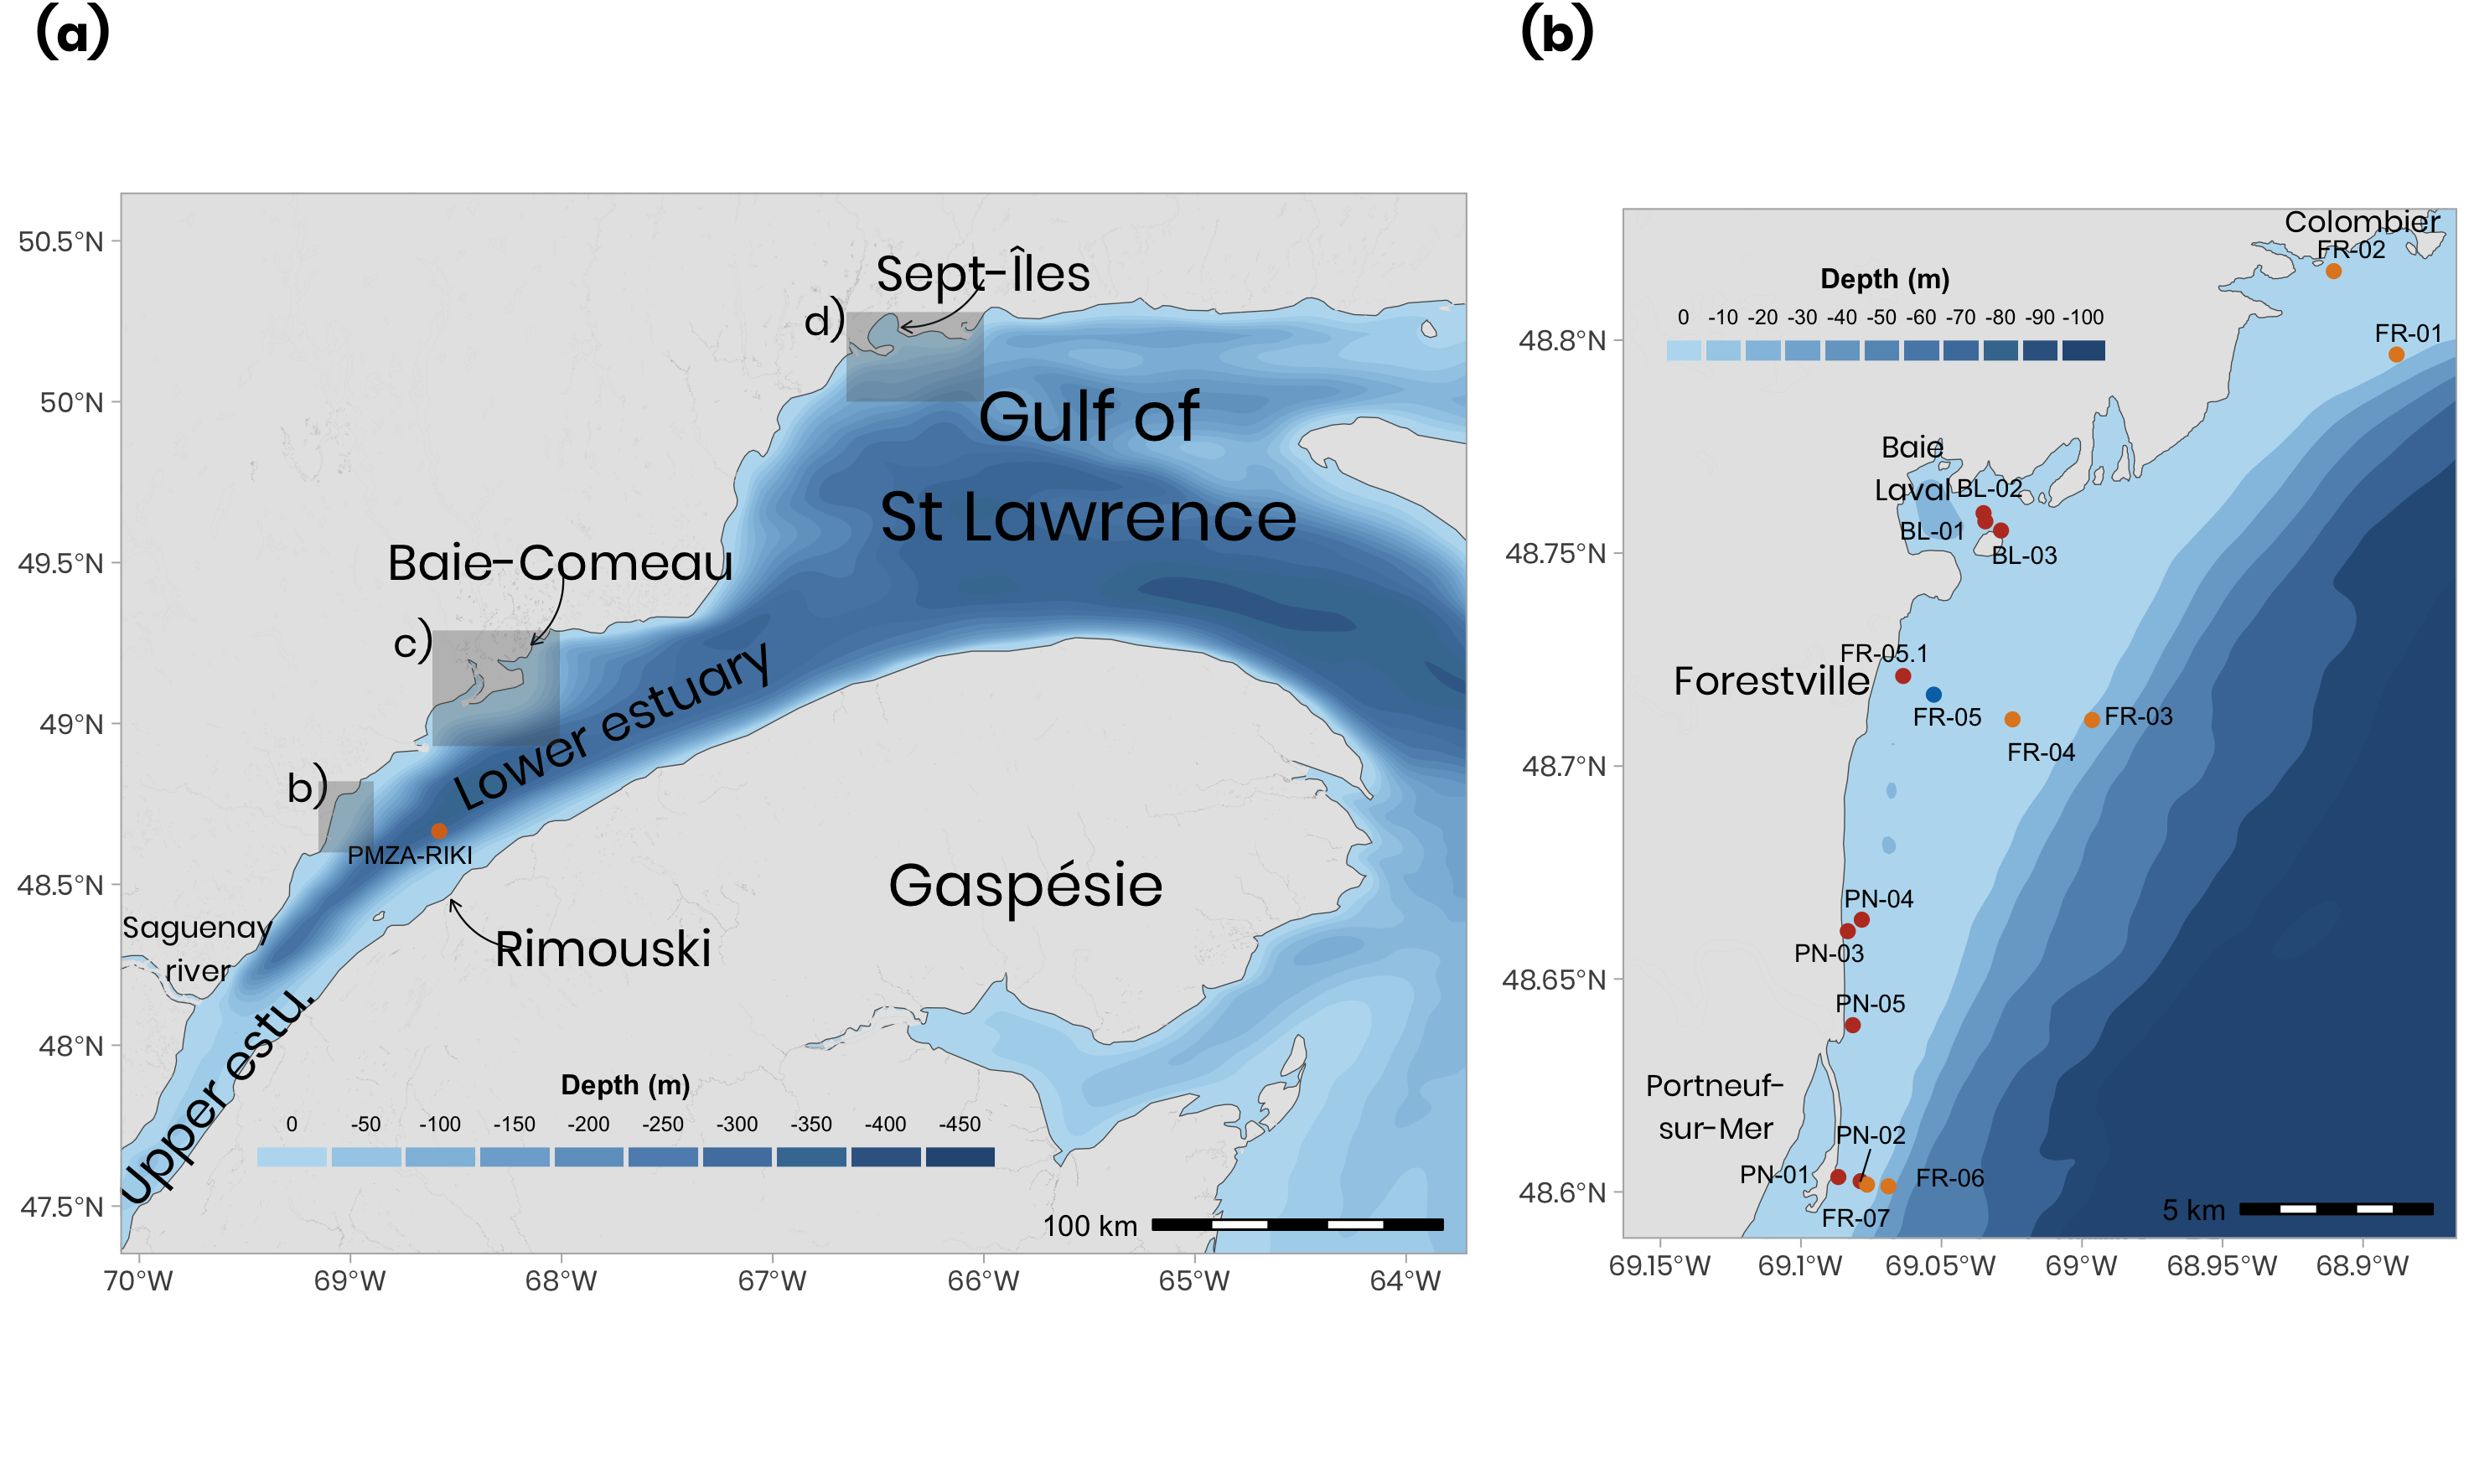
\includegraphics[width=12cm]{Figures/Fig1a-b.png}
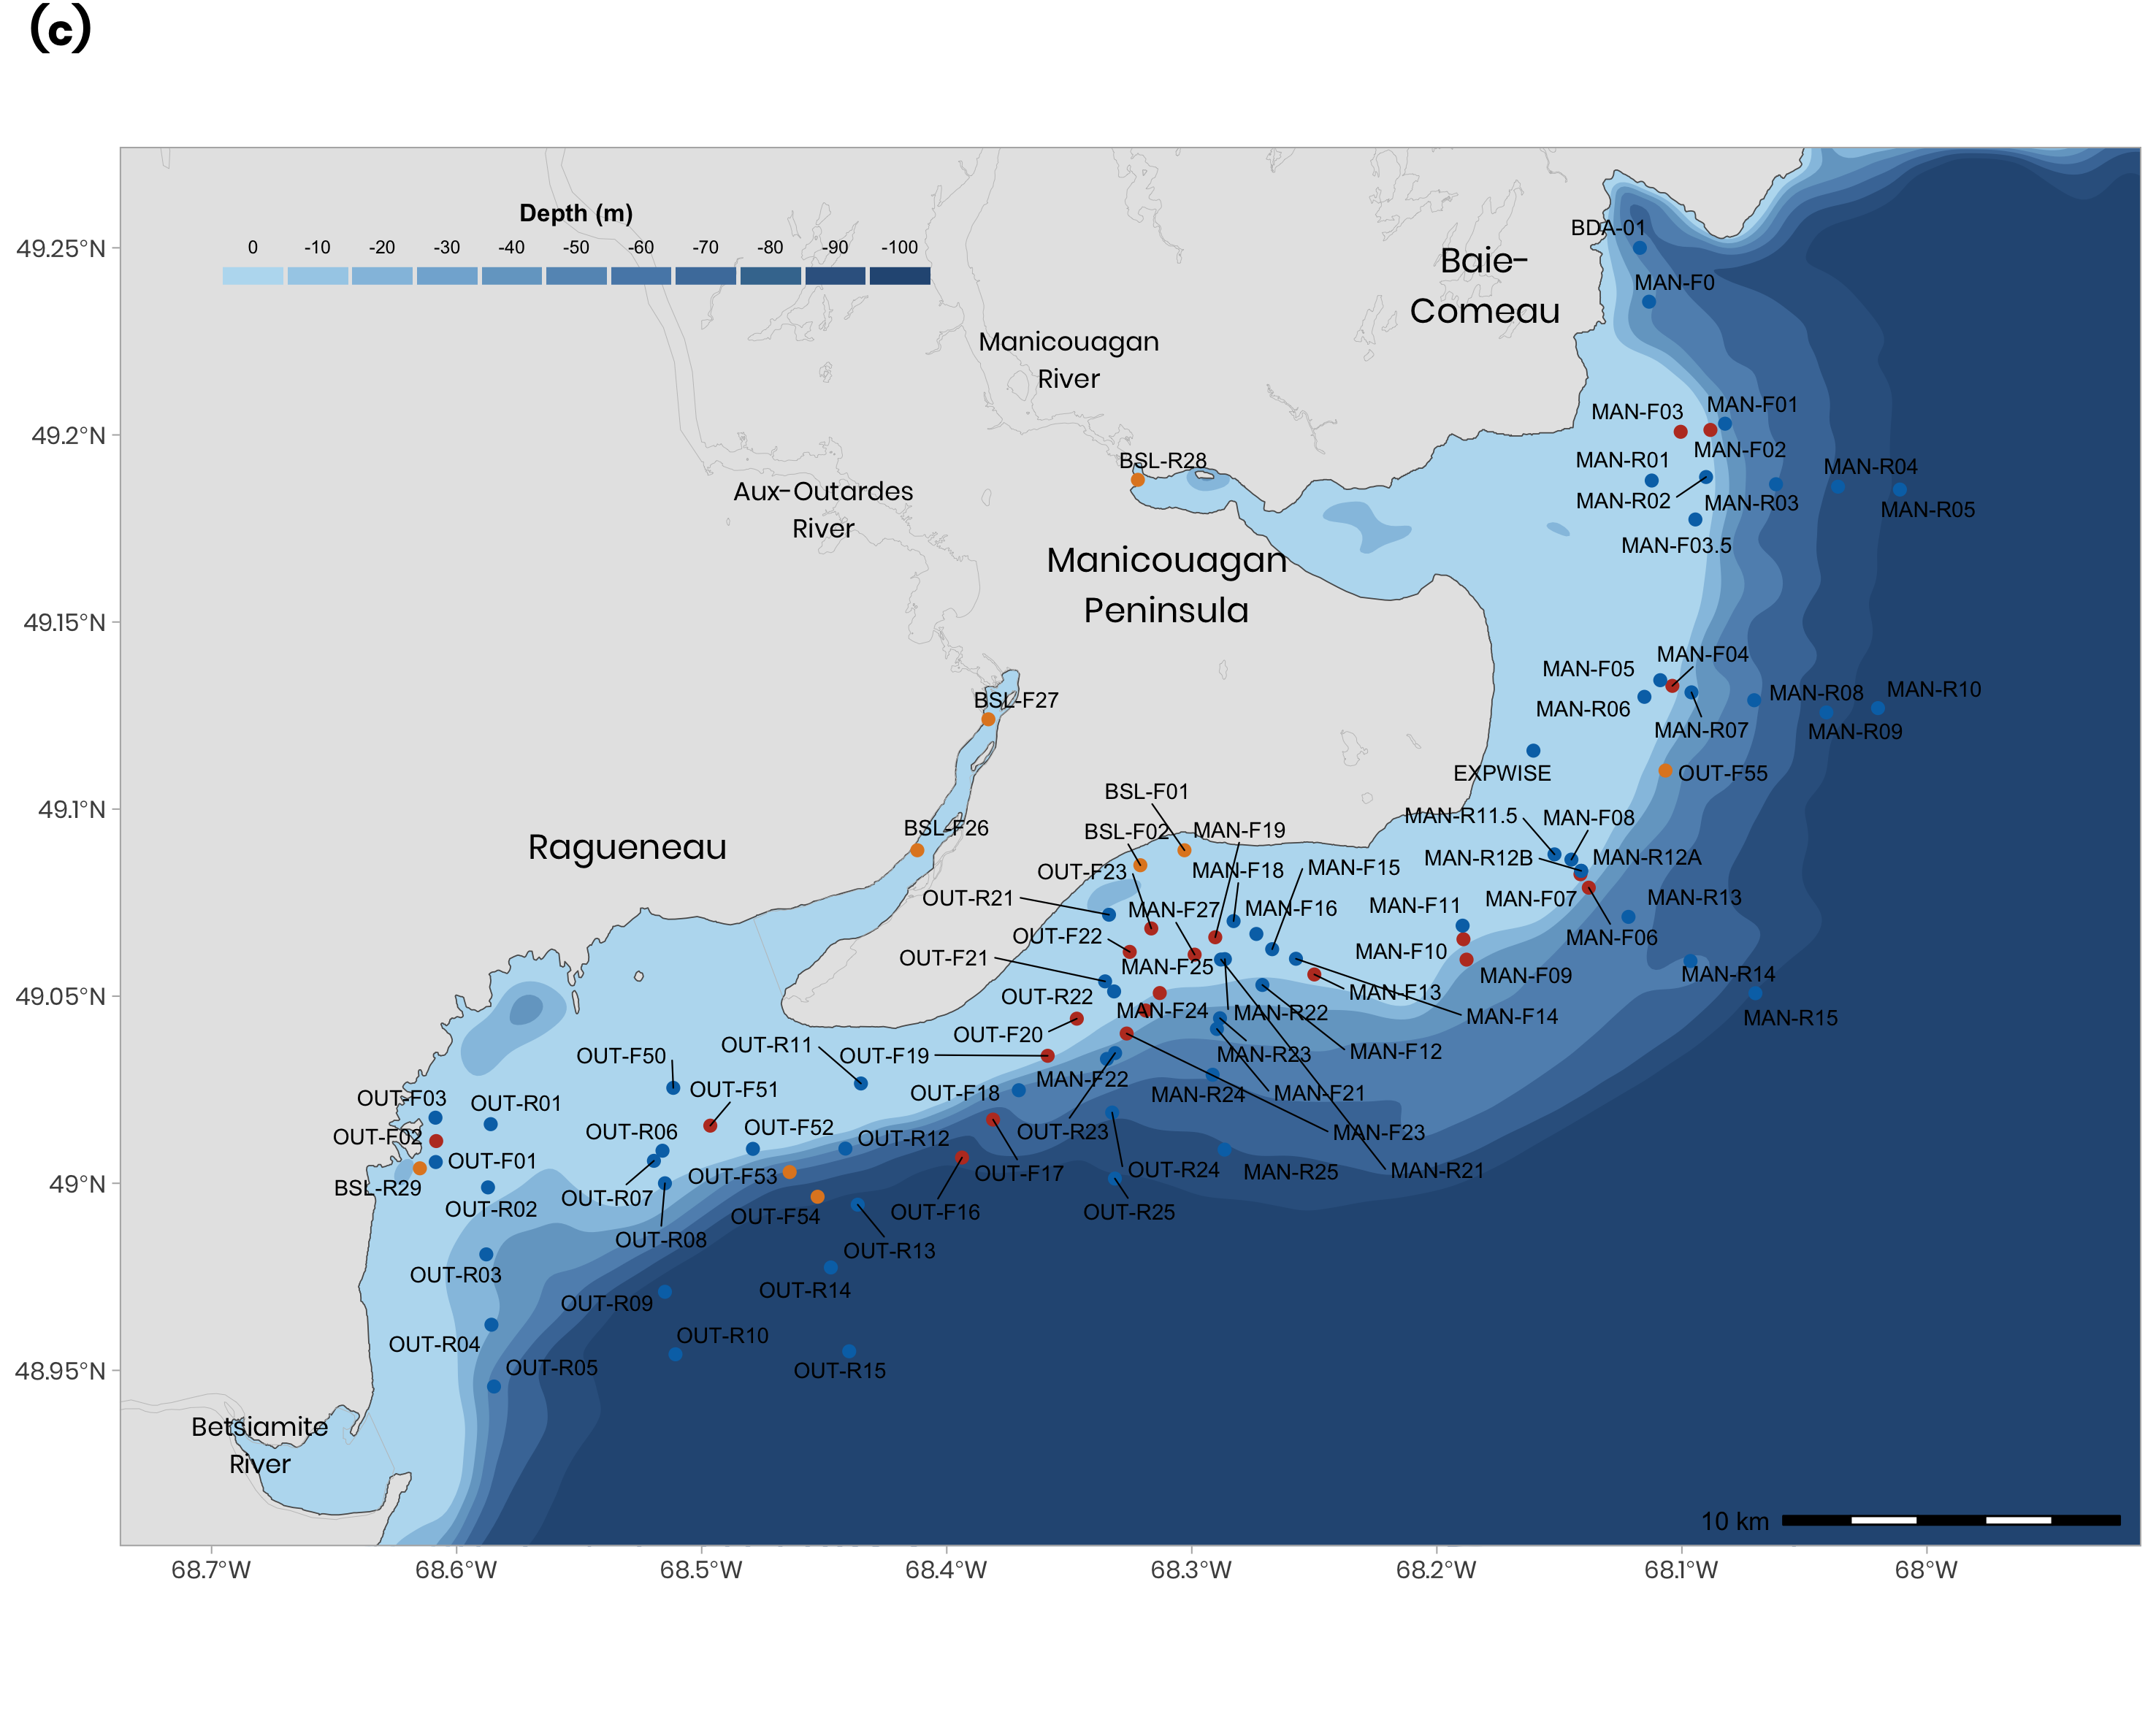
\includegraphics[width=12cm]{Figures/Fig1c.png}
\caption{Maps of stations where apparent optical properties (AOPs) have been determined. Insets in (a) are presented in (b) for the Forestville-Portneuf-sur-mer area visited on September 11 2017, (c) the Manicouagan Peninsula visited in August 2019, and (d) the Sept-Iles area visited on 11 occasions between August 2016 and June 2019. The color points indicate how the remote sensing reflectance was measured: in-water only (orange), above-water only (red) or both methods (blue).}
\label{fig:maps}
\end{figure}
\setcounter{figure}{0}
\begin{figure}[!ht]
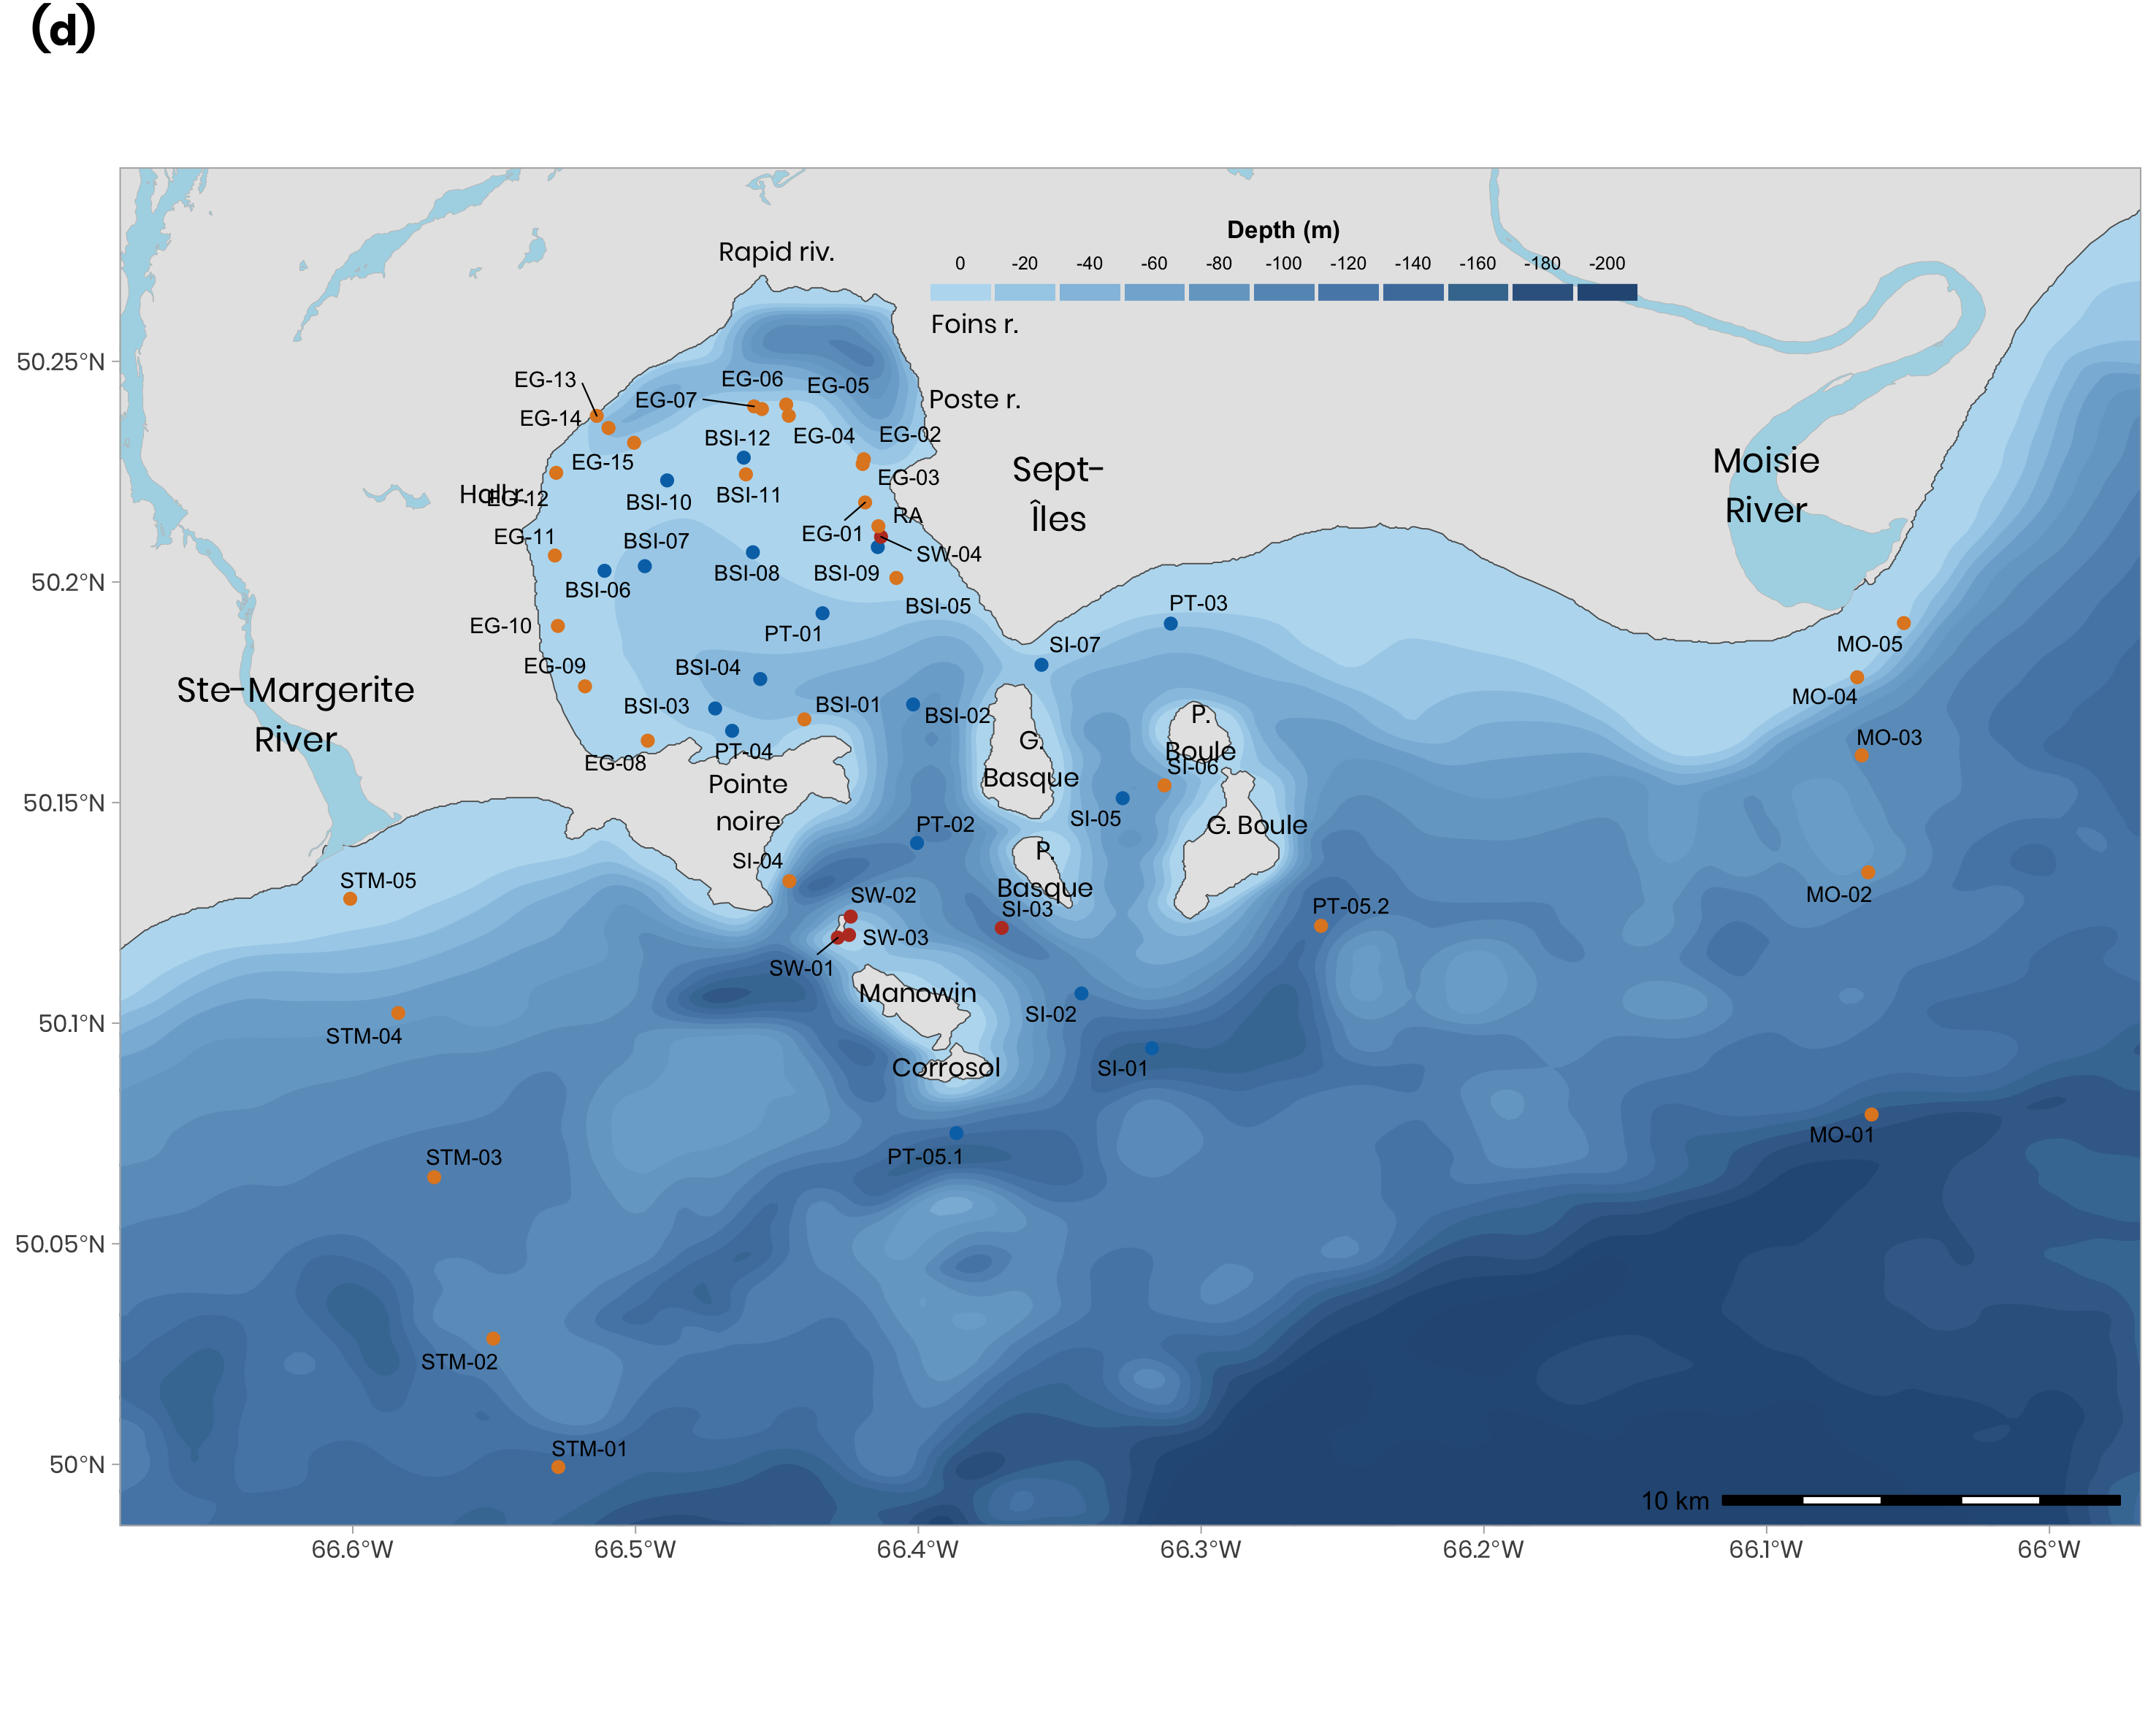
\includegraphics[width=12cm]{Figures/Fig1d.png}
\caption{Continue}
\end{figure}

\subsection{Optical buoy of the Atlantic Zone Monitoring Program (AZMP): St Lawrence marine estuary}
The Atlantic Zone Monitoring Program (AZMP), or Programme de Monitorage de la Zone Atlantique (PMZA) of DFO includes a network of autonomous oceanographic buoys across the coastal waters of the Maritime provinces of Canada. The station named PMZA-RIKI (Figure~\ref{fig:maps}a) in the SLE, in front of Rimouski, has been visited on a regular basis (once a week in summer) since 1991. It was the first station to be instrumented with an autonomous buoys in 2002, including multispectral sensors dedicated to satellite validation of radiometric products. In 2015, a project was put in place to assess the quality of the radiometric quantities available at the station PMZA-RIKI with the goal to use these data for the validation of operational Sentinel-3 radiometric products \citep{Belanger2017}. The station was visited on 19 occasions between June 3rd and November 5th 2015, three times in 2016 (August 11 and 19, Sept 16) and once in 2017 (May 17) onboard DFO small (i.e. 30-foot length) craft boats (Table \ref{table:datasummary}).  On each occasion, 3 to 5 light profiles were carried with a Compact-Optical Profiling System (C-OPS) next to the buoy to determine the AOPs. An optical package, which included a CTD (conductivity-temperature-depth; SBE19 from Seabird scientific) and various optical instruments (Hydroscat-6p, a-sphere, ECO-triplet), was also deployed for the determination of inherent optical properties (IOPs). After the deployment of the instrumentation near the buoy, surface waters were sampled using a clean 20-L carboy kept in an iced cooler until it was processed in the Université du Québec à Rimouski (UQAR) laboratory later that same day. Several physicochemical (e.g., total suspended solids (TSS), dissolved organic carbon (DOC), salinity, nutrients), biological (chlorophyll-a, pigments, bacterial and phytoplankton cell counts) and optical parameters were determined from the discrete water samples. This data set was partially presented in \citet{Belanger2017} where more details about the sampling strategy can be found. Unlike most coastal stations located along the northern shore of St Lawrence presented below, the estuarine waters found at the PMZA-RIKI station is under the influence of the St Lawrence river and the up-welling of deep water taking place a the head of the Laurentian Channel near Tadoussac at the mouth of the Saguenay Fjord (Figure~\ref{fig:maps}a). This increases the range of optical conditions encountered in the actual nearshore data set.   
 
\begin{table}[t]
\caption{Summary of field campaigns.}
\centering
\begin{tabular}{ p{3cm}|p{3cm}|c|p{1.5cm}|c|p{1.5cm}p{1.5cm}p{1.5cm}p{1.5cm}|p{1.5cm}p{1.5cm}p{1.5cm}p{1.5cm}p{1.5cm}  }
\tophline
Area & Research project & Year & Number of campaigns & Dates &
\multicolumn{4}{c|}{Number of stations} &
\multicolumn{5}{c}{Number of measurements}\\
\middlehline
 & & & & & Sea & River & Intertidal & Infralittoral & In-water radiometry & Above-water radiometry & IOPS packae & Surface water samples & Sub-surface water samples \\
\middlehline
Rimouski (PMZA-RIKI estuary station) & Atlantic Zone Monitoring Program (AZMP) & 2015 & 18 & June 3 to Nov 5 & 1 & NA & NA & NA & 18 & 0 & 12 & 19 & 0\\
& & 2016 & 2 & Aug 11 and 19 & 1 & NA & NA & NA & 3 & 0 & 0 & 0 & 0\\
& & 2017 & 1 & May 17 & 1 & NA & NA & NA & 1 & 0 & 1 & 0 & 0\\
\middlehline
Baie of Sept-Iles (BSI) & CHONe & 2016 & 1 & Aug 23 and 24 & 9 & 3 & NA & NA & 9 & 0 & 0 & 12 & 0\\
 & & 2017 & 9 & Apr 10 to Oct 9 & 26 & 5 & NA & NA & 63 & 0 & 54 & 101 & 9\\
 & & 2019 & 1 & June 1 to 5 & 40 & 5 & NA & NA & 32 & 0 & 23 & 42 & 0\\
 & microCASI & 2017 & 1 & Sept 14 & 26 & 0 & NA & NA & 7 & 10 & 7 & 6 & 0\\
\middlehline
Forestville-Portneuf-sur-mer & microCASI & 2017 & 1 & Sept 11 & 16 & NA & NA & NA & 7 & 10 & 7 & 6 & 0\\
\middlehline
Manicouagan & WISE-Man & 2019 & 1 & Aug 17 to 25 & 89 & 3 & 195 & 7 & 59+dive? & 84+195+dive? & 63 & 70 & 15\\
\bottomhline
 \end{tabular}
 \label{table:datasummary}
\end{table}


\subsection{Canadian Healthy Ocean Network (CHONe-2): Baie of Sept-Îles (BSI) project}
Within the scope of CHONe-2 funded by the Natural Sciences and Engineering Research Council of Canada (NSERC), 11 field campaigns were conducted in the Bay of Sept-Iles area from August 2016 to June 2019 (Figure~\ref{fig:maps}d, Table \ref{table:datasummary}).  The general objective of the CHONe-2 project in the BSI was to assess the potential stress of industrial and port activities on the coastal ecosystem, including vegetated habitats (eelgrass meadows and macroalgae), and benthic and pelagic ecosystems \citep{Ferrario2021}. One of the goal was to establish a bio-optical data baseline to promote and develop optical remote sensing tools for monitoring purposes, at the bay scale \citep{Araujo2022}.

Between 12 and 45 stations were visited on a given year in the BSI area (Table \ref{table:datasummary}). Bio-optical data was gathered both inside and outside the BSI, as well as on five rivers: four inside (Hall, au Foin, des Rapides and Poste) and one outside (Moisie) the bay (Figure~\ref{fig:maps}d).  Typical measurements at sea involved radiometric measurements for AOPs (C-OPS) and IOPs profiles (same optical package as above) and water sampling for laboratory analysis. The water sampling at sea was taken mostly at the surface using a bucket, but in 2017 some subsurface water samples were also taken using niskin bottles to compare the phytoplankton community living in the subsurface chlorophyll-a maximum. The sampling at sea was made on a fisherman boat based at the Sept-Iles port. Rivers were accessed by foot from the main roads and measurements were made with a multiparameter probe and surface water was collected for laboratory analysis.

AOPs and IOPs, as well as water sample parameters measured, varied from one station to another mainly because of instrument availability.   Overall, a total of 56 unique sea stations and 5 river stations were repeatedly visited from 2016 to 2019. As a results, 104 measurements were made at sea for AOPs and 164 water samples (155 surface, 9 subsurface) were analysed for physico-chemical and bio-optical parameters. Details are presented in Appendix xx and in \citet{Araujo2022}.

%For the nearshore vegetation, with a focus on the eelgrass (\textit{Zostera marina, L.}), the campaign conducted in late June 2017 gathered above-water radiometry data (n = ???) concomitantly with a single-beam acoustic survey, using a small boat adapted for very shallow waters. Complementary, a dedicated campaign in July 2017 was made to gather reflectance spectra (n =xx?) in the canopy of the eelgrass meadows, during low tide conditions.

\subsection{Hyperspectral remote sensing of optically shallow and coastal waters: microCASI and WISE-Man projects}
In September 2017, with the collaboration of DFO and the Canadian Hydrographic Service (CHS), fieldwork in support of airborne hyperspectral imagery acquisition was carried along the northern shore of the EGSL. The main objective of these acquisitions was to map the nearshore coastal ecosystems (e.g.m eelgrass meadows, macroalgae, saltmarsh) and derived bathymetry. The microCASI sensor was flown on September 11 by the IIC company in the Forestville area (Figure~\ref{fig:maps}b) and on September 14, and in the BSI (Figure~\ref{fig:maps}d). The stations in the BSI were sampled as part of the CHONe-2 field campaigns described above (n = 26 stations, Table \ref{table:datasummary}). In Forestville,  a total of 16 stations were visited (Table \ref{table:datasummary}). Above-water radiometry was measured using an ASD spectroradiometer at 16 stations (6 in BSI and 10 in Forestville, Table \ref{table:datasummary}), Figure~\ref{fig:maps}b) with a small zodiac. In-water radiometry with the C-OPS was performed at 16 stations (9 in BSI and 7 in Forestville) and surface water was sampled at 12 of them (6 in BSI and 6 in Forestville) for basic bio-optical and biogeochemical parameters, i.e. TSS, fluorometric chlorophyll-a concentration, CDOM and particulate absorption coefficients.
 
In August 2019, an intensive field campaign was organized in the frame of the WaterSat Imaging Spectrometer Experiment (the \textit{WISE-Man project}; \textit{Man} stands for \textbf{Man}icouagan) in collaboration with several federal departments (DFO, NRC, DRDC) and university (UQAC, Laval). %a project supported by the Flights and Fieldwork for the Advancement of Science and Technology (FAST) program of the Canadian Space Agency (CSA), the Réseau Québec Maritime (RQM) and the DFO Ocean Protection Plan baseline program.  
The WISE-Man main's objective was to demonstrate the potential of hyperspectral imagery for mapping bathymetry, water column quality (or IOPs), and retrieve bottom properties in order to respond to the pressing needs of science (e.g. ecology, geomorphology, coastal risk), resource management and defense operations.  In particular, the goal was to assess the performance of the WISE camera, a prototype sensor developed by ITRES inc. (Calgary, Canada) within the framework of the Canadian Space Agency (CSA) initiative called WaterSat. 
 
The WISE-Man fieldwork campaign was conducted in the Manicouagan Peninsula, near Baie-Comeau, along the northern shore of the St Lawrence Estuary (Figure~\ref{fig:maps}c). A total of 92 stations were visited between August 17 and 25 2019 for AOPs determination (at least for the remote sensing reflectance) using four small boats (Table \ref{table:datasummary}). Figure~\ref{fig:maps}c distinguishes the stations visited during the WISE flights of the 18 and 20 of August (e.g., MAN-Fx, OUT-Fx) from those visiting the other days (e.g. MAN-Rx, OUT-Rx). At 64 out of 92 stations, CTD and \textit{in situ} IOPs were measured using two different instrument set-ups, and surface water was sampled using either a 5 L Niskin or a 4.2 L Wildco Beta horizontal sampler fired at about 0.5 m (surface; N = 64) or 4 to 5 m depth (sub-surface; N = 15, Table \ref{table:datasummary}). Two stations were sampled twice for water (EXPWISE and BDA-01) and six additional stations were sampled directly at the surface using a 20-L carboy from a small zodiac, for a total number of 85 discrete water samples for the whole mission (Table \ref{table:datasummary}). 
 
During WISE-Man, inter-tidal (0-2 meters below sea level) and infra-littoral (2-5 m depth) fieldwork was also undertaken to characterize the sea bottom habitats. The inter-tidal zone was characterized at low tide between July 27 and August 8, 2019 at  195 stations (Figure~\ref{fig:intertidal}, Table \ref{table:datasummary}). A SCUBA diving team performed ten transects at seven locations in the infra-littoral zone.  In addition to the hyperspectral reflectance measurement (emerged or submerged), ecological, biological and physicochemical observations were performed.  

\begin{figure}
    \centering
    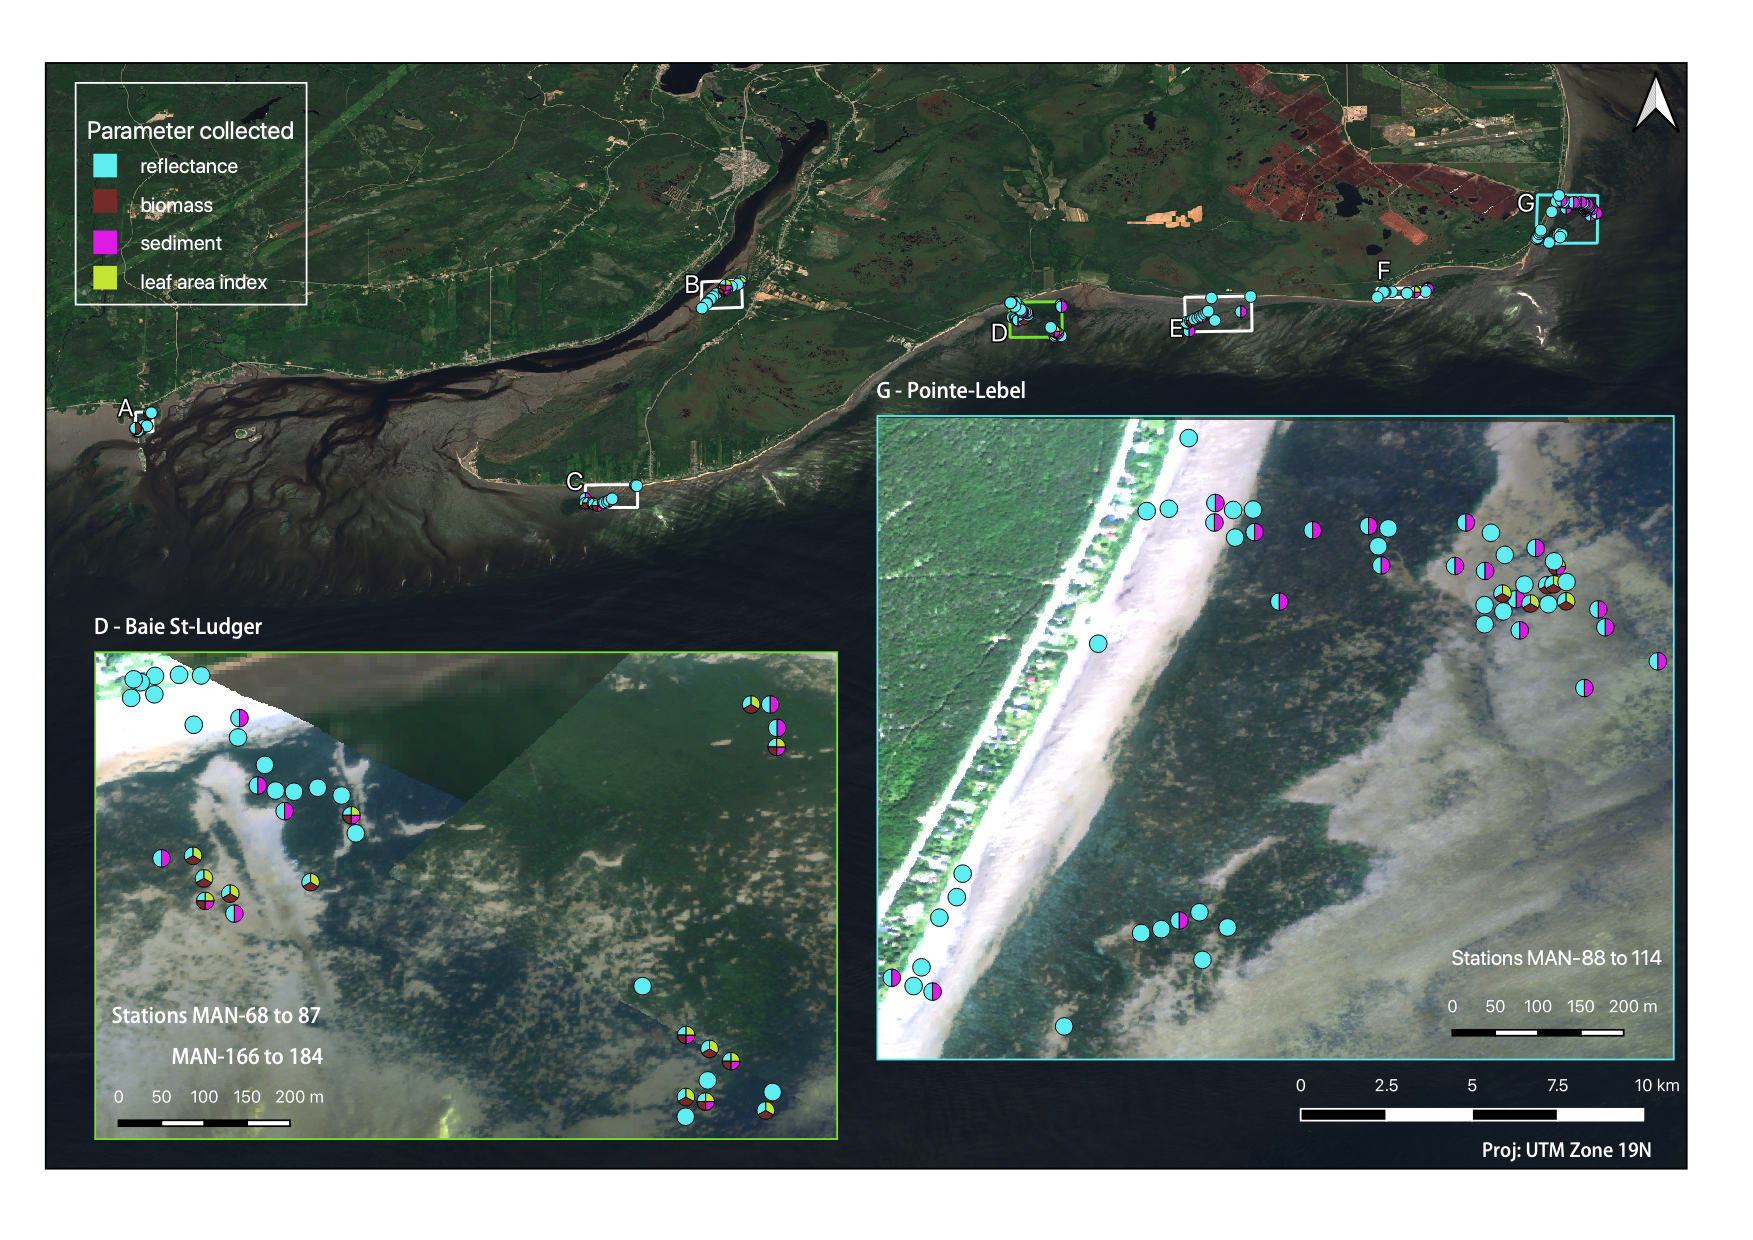
\includegraphics[width=18cm]{Figures/Fig2_intertidal_v3.png}
    \caption{Map of stations in the inter-tidal zone visited at low tide between July 27 and August 8, 2019 in the Manicouagan peninsula, showing the different parameters sampled. . Insets are zoomed in for two sectors (D and G) out of seven (maps for sectors A,B,C,E and F are available in Appendix ~\ref{appendixfig}. }
    \label{fig:intertidal}
\end{figure}


\section{Material and methods}
This section provides a detailed description of the material and methods (M\&M) adopted for \textit{in situ} observations at each station (section~\ref{insitu}, including, AOPs IOPs and sun photometry), biogeochemical parameters on discrete water samples (section~\ref{labo}) and benthic habitats characterization (section~\ref{benthos}). Most M\&M are common to all projects presented above, but any project-related differences are pointed out below. 

\subsection{In situ observations on stations} \label{insitu}
At a typical station, the following operations were performed at sea (note: the actual order may change depending on the time of the day or the sea state):
\begin{itemize}
  \item Three to five vertical profiles are done with the C-OPS for AOPs  determination.
  \item One vertical profile is made with an instrument package that includes at least a CTD and various active optical sensors for IOPs determination.
  \item When available, additional vertical profiles are made for multiparametric measurements (e.g., CTD, in vivo chlorophyll fluorescence, CDOM fluorescence, pH, oxygen, turbidity, etc).
  \item Wind speed and direction is recorded for later processing. 
  \item When available and under clear sky, sun photometry is performed using a Microtops to determine the atmospheric aerosol optical depth and water vapor content (WISE-Man only).
  \item Surface water (~ 20-L), and on some occasions sub-surface water, is sampled using a bucket or a water sampler such as a Niskin bottle fired at 0.5 m depth. The water sample is kept in the dark in a cooler until it is processed in the laboratory within 12 hours after sampling.
\end{itemize}

\subsubsection{Radiometric measurements and AOPs}
AOPs are those properties that are determined using radiometric measurements and that depend upon the ambient light field, the IOPs and the boundary conditions (sea state and bottom reflectance) \citep{Preisendorfer1961}.  Some of them, such as the diffuse attenuation coefficient of downwelling irradiance ($K_d$) can only be determined from in-water vertical light profiles, while others, such as the remote sensing reflectance $R_{rs}$, can be determined using radiometric measurements made in-water or above-water.  Here we describe both approaches and give the main particularities of each instrument employed to determine the AOPs in our data set.\\  

\textbf{C-OPS}\\
The main instrument used to determine in-water AOPs, common to all projects, is the C-OPS. All together, the data set contains 216 different stations totalizing about 1000 C-OPS profiles. The C-OPS measures the light field in the water column with very high precision and accuracy at a frequency of 15 Hz \citep{Hooker2013, Morrow2010}. The UQAR C-OPS (Biospherical Instruments) measures the downwelling irradiance and the upwelling radiance in the water column at 19 wavebands ($\lambda$), i.e. $E_d(z,\lambda)$ and  $L_u(z,\lambda)$) where $z$ is depth. Simultaneous above-surface downward irradiance ($E_d(0+, \lambda)$) was measured with a radiometer attached on top of the boat making sure that no obstructions were in the field of view. In 2017, a new frame was purchased to deploy a third in-water sensor for upwelling irradiance, $E_u(z,\lambda)$. The wavebands for the UQAR C-OPS are presented in Table~\ref{table:COPSwave} (note that the 305 nm channel was replaced by a 875 nm channel before the 2016 field season).  In 2019, the C-OPS from Boston University (Dr Cedric Fichot) was used during the WISE-Man mission (35 stations), which has 16 common channels with the current UQAR instrument setting (Table~\ref{table:COPSwave}). 

\begin{table}[t]
\caption{Wavebands available on the two C-OPS systems.}
\centering
\begin{tabular}{ m{2.5cm}m{2.5cm}|m{2.5cm}  }
\tophline
\multicolumn{2}{c|}{UQAR SN 13} &
Boston University \\
\middlehline
2015 & 2016-2019 & 2019 \\
\middlehline
305  & NA  & 305 \\
320 & 320 & 320 \\
330 & 330 & NA \\
340 & 340 & 340 \\
380 & 380 & 380 \\
NA & NA & 395 \\
412 & 412 & 412 \\
443 & 443 & 443 \\
465 & 465 & 465 \\
490 & 490 & 490 \\
510 & 510 & 510 \\
532 & 532 & 532 \\
555 & 555 & NA \\
NA & NA & 560 \\
589 & 589 & 589 \\
625 & 625 & 625 \\
665 & 665 & 665 \\
683 & 683 & 683 \\
694 & 694 & 694 \\
710 & 710 & 710 \\
780 & 780 & 780 \\
NA & 875 & NA \\
\bottomhline
 \end{tabular}
 \label{table:COPSwave}
\end{table}

As mentioned above, three to five C-OPS profiles were performed on each station. Most of the time, the boats were drifting during the measurements and the instrument was kept outside any disturbance or boat shadow. In very shallow waters (z $<$ 2 m) where tidal currents were strong, the boats were anchored to stay on station and the instruments were transported away from the boat shadows. 
 
The C-OPS data were processed in R software with the \texttt{Cops} package first developed by Dr. B. Gentili at the Laboratoire d'Océanographie de Villefranche (LOV) and now maintained by Dr S Bélanger (the source code is available at \url{https://github.com/belasi01/Cops}). The data processing respects the NASA protocols \citep{Mueller2003vIII} but additional features have been developed to optimized the data processing. AOPs were derived from vertical profiles of downward irradiance ($E_d(z,\lambda)$), upwelling radiance ($L_u(z,\lambda)$) and when available, upwelling irradiance ($E_u(z,\lambda)$). Each profile was carefully inspected and records showing high instrument tilt were discarded, i.e. $> 5^{\circ}$ for in-water and $> 10^{\circ}$ for $E_d(0+,\lambda)$. As the tilt is often high in surface water, highly stratified or shallow waters, we often have to relax the tilt limit threshold to 7 or 8 $^{\circ}$ for the upwelling quantities (i.e., $E_u(z,\lambda)$ and $L_u(z,\lambda)$) to keep enough data points in the first-meter of water to obtain a precise extrapolation of the radiometric quantities at the sea-air interface ($z=0-$). In addition, radiometric quantities below the instrument detection limit were removed (i.e., noisy measurements). The later varies between instruments and wavebands. Typical values for the detection limit vary from \num{1e-4} to \num{7e-3} \si{\micro.W.cm^{-2}.nm^{-1}} for $E_d(z,\lambda)$ and $E_u(z,\lambda)$, and for \num{1e-5} to \num{2e-4} \si{\micro.W.cm^{-2}.nm^{-1}.sr^{-1}} for $L_u(z,\lambda)$. The detection limit is lowest in the visible bands and highest in the UV domain. In CDOM-rich waters, such as those characterizing the nearshore waters of the EGSL, the detection limit is often reached in the top 10 meters in the UV channels.\\ 

In-water radiometric quantities ($E_d(z,\lambda)$, $E_u(z,\lambda)$ and $L_u(z,\lambda)$) were normalized with respect to simultaneous measurements of the global solar irradiance in the air, $E_d(0+,\lambda,t)$, with $t$ explicitly expressing the time dependence, according to

\begin{equation}
\Xi(z,\lambda,t_0) = \Xi((z,\lambda,t))\frac{E_d(0+,\lambda,t_0)}{E_d(0+,\lambda,t)}
\label{eq:xi}
\end{equation}

where $\Xi$ identifies the radiometric quantity that is normalized to account for incident irradiance fluctuations during the vertical profiles induced by the atmospheric conditions. After the normalization and filtering of $\Xi$, the data are fitted using a linear regression applied to log-transformed radiometric quantity versus depth allowing extrapolation of the quantities of interest just below the sea surface ($z=0-$). A non-linear fitting method was also implemented in the Cops R package, known as LOESS (local polynomial regression fitting), which is a non-parametric method usually employed to smooth time-series (but here applied to light profile). LOESS computes polynomials on the data for a given moving window size (typically 3 to 5 meters) along the profile. The LOESS fitting is particularly efficient for smoothing $\Xi$ profiles showing actual non-linear features introduced by either non-homogenous vertical profile, the presence of bottom in optically shallow waters or the effect of inelastic scattering processes (e.g., sun-induced fluorescence in subsurface chlorophyll-a maximum layers).  It could also be used to extrapolate $\Xi$ to $z=0-$. 

The thickness of the surface layer considered for the $\Xi(z,\lambda,t_0)$ linear extrapolation varied as a function of wavebands and the quality of the data fitting. It varied between 0.3 and 2.5~m (3.0 for $E_d(z,\lambda)$) below the very first C-OPS measurements in the water column (typically around 0.35 to 0.5~m depth). For example, if C-OPS measurements begin at 0.4 m, the minimum layer considered will extend from 0.4 to 0.7~m and the maximum layer from 0.4 to 2.9~m. A linear model is fitted to the log-transformed $\Xi(z,\lambda,t_0)$ vs depth ($z$) to all layers from the minimum and the maximum thickness considered, starting with a minimum number of ten valid measurements and adding one observation at a time. The goodness of the fit is evaluated using the coefficient of determination ($r^2$) to all layers. In addition, we apply a Kolmogorov-Smirnov test to make sure the depth distribution within each layer is not bimodal, which can produce a high value of $r^2$. It compares the actual $z$ distribution to an expected $z$ distribution, in which $z$ is evenly spaced from the minimum and maximum depth the layer considered. If the p.value $>$ 0.1, the $z$ distribution is considered not evenly spaced and the fit is not retrained (even if it presents the highest $r^2$). Otherwise, the layer presenting the highest $r^2$ is retrained for the linear extrapolation of $\Xi(z,\lambda,t_0)$. Finally, we imposed arbitrarily a lower limit for the $r^2$ of 0.6 for $E_u(z,\lambda)$ and $L_u(z,\lambda)$) and 0.5 for $E_d(z,\lambda)$. Noisy data due to wave focusing effect may result in a failure of the linear extrapolation. In general, the thickness of the layers considered are thinner in the UV and near-infrared spectral domains. This method is similar to that adopted by \citet{Antoine2013a} and is improved relative to that described in \citet{Belanger2017}. 

$L_u(0-,\lambda)$ and $E_u(0-,\lambda)$ were corrected for instrument self-shadow following the procedure proposed by \citet{Gordon1992b} and \citet{Zibordi1995}, which requires the total absorption coefficients, $a_t$, at each C-OPS channels. For most station, \textit{in situ} non-water absorption profiles were used. Otherwise, discrete measurements of CDOM and particulate absorption coefficients were used. In the rare case where \textit{in situ} and discrete absorption measurements were not available, total absorption was estimated from diffuse downwelling attenuation coefficient ($K_d$) and the sub-surface irradiance reflectance ($R$) computed for the surface layer using the analytical model described in \citet{Morel2001} (their eq. 8').\\ 
Water-leaving radiance, $L_w(\lambda)$, was calculated from the extrapolated upwelling radiance just below the sea surface as:
 \begin{equation}
 \label{eq:L_w}
L_w(\lambda) = 0.54\,L_u(0-,\lambda)
\end{equation}
where the factor 0.54 accounts for the partial reflection and transmission of the upwelled radiance through the sea surface. 
The remote sensing reflectance, $R_{rs}(\lambda)$, was computed as:
 \begin{equation}
 \label{eq:Rrs}
R_{rs}(\lambda) = \frac{L_w(\lambda)}{E_d(0+,\lambda,t_0)} 
\end{equation}

For a given date, the AOPs derived from three to five profiles were averaged after eliminating spectra that showed large discrepancy relative to the mean spectrum (i.e., if the difference between mean and replicates was $>$10\% in terms of $R_{rs}$).\\  

The AOPs data set also includes spectral diffuse attenuation coefficient of downwelling irradiance, $K_d(\lambda)$, as computed for two surface layers. Here we defined an average attenuation coefficient from the surface (0-) to the depth $z$ where the downwelling irradiance is reduced to 10\% or 1\% of its surface value measured just below the sea surface (i.e., $E_d(0-)$):  

\begin{equation}
    \overline{K_d}(0- \leftrightarrow z) = \frac{1}{z}\ln \left( \frac{E_d(z)}{E_d(0-)} \right)
    \label{eq:Kd}
\end{equation}

Therefore, $\overline{K_d^{1\%}}$ and $\overline{K_d^{10\%}}$ were computed using eq~\ref{eq:Kd} for the depth $z$ where $\frac{E_d(z)}{E_d(0-)}$ yield a values of 1\% and 10\%, respectively. The calculation is based on $E_d(0-)$ obtained from measured $E_d(0+)$ times 0.97 to account for the air-sea transmittance \citep{Mueller2003vIII} and vertical profiles of normalized $E_d(z)$ (eq.~\ref{eq:xi}) and smoothed using the LOESS fitting method. As a result, the depth of the actual layer consider for $\overline{K_d}$ is wavelength dependent since the depth of the 1\% or the 10\% light level is spectrally dependent. \\ 

In optically shallow waters the bottom reflectance, $R_b$,  can be extracted from C-OPS profiles if the light intensity is above the detection limit when the instrument reach the bottom of the water column. Figure~\ref{fig:Rb} presents an example of a C-OPS profile performed in the eastern side of Manicouagan Peninsula over a sandy bottom. First, the depth of the water column is estimated using the pressure sensor of the C-OPS. In this example, the instrument was free falling from the surface to the bottom when the pressure remained constant at 5.2~m (Figure~\ref{fig:Rb}a), yielding a total water column depth of 5.45~m after adding the distance between the pressure sensor and the base of the instrument (0.25~m). All radiometric data in the first 15~cm above the bottom are contaminated by instrument shading and are systematically removed. Figures~\ref{fig:Rb}b and \ref{fig:Rb}c show the vertical profiles of $E_d(z)$ and $L_u(z)$, respectively, at three selected wavelengths in the visible (i.e., 443, 560 and 625 nm). While $E_d(z)$ show a typical exponential decrease with depth at all wavelengths,  $L_u(z)$ in the blue tend to level off at 3~m, and even increase slightly with depth in the green and in the red due to the bottom reflectance, which is higher than the water column reflectance itself. The bottom reflectance ($R_b$) is estimated using the radiometric quantities measured 25~cm above the bottom (i.e., dashed grey lines on Figures\ref{fig:Rb}b and c).

\begin{equation}
    R_b = \frac{\pi \times L_u(z = \mathrm{bottom-0.25~m})}{E_d(z = \mathrm{bottom-0.25~m})} = \frac{E_u(z = \mathrm{bottom-0.25~m})}{E_d(z = \mathrm{bottom-0.25~m})}
\end{equation}

\begin{figure}
    \centering
    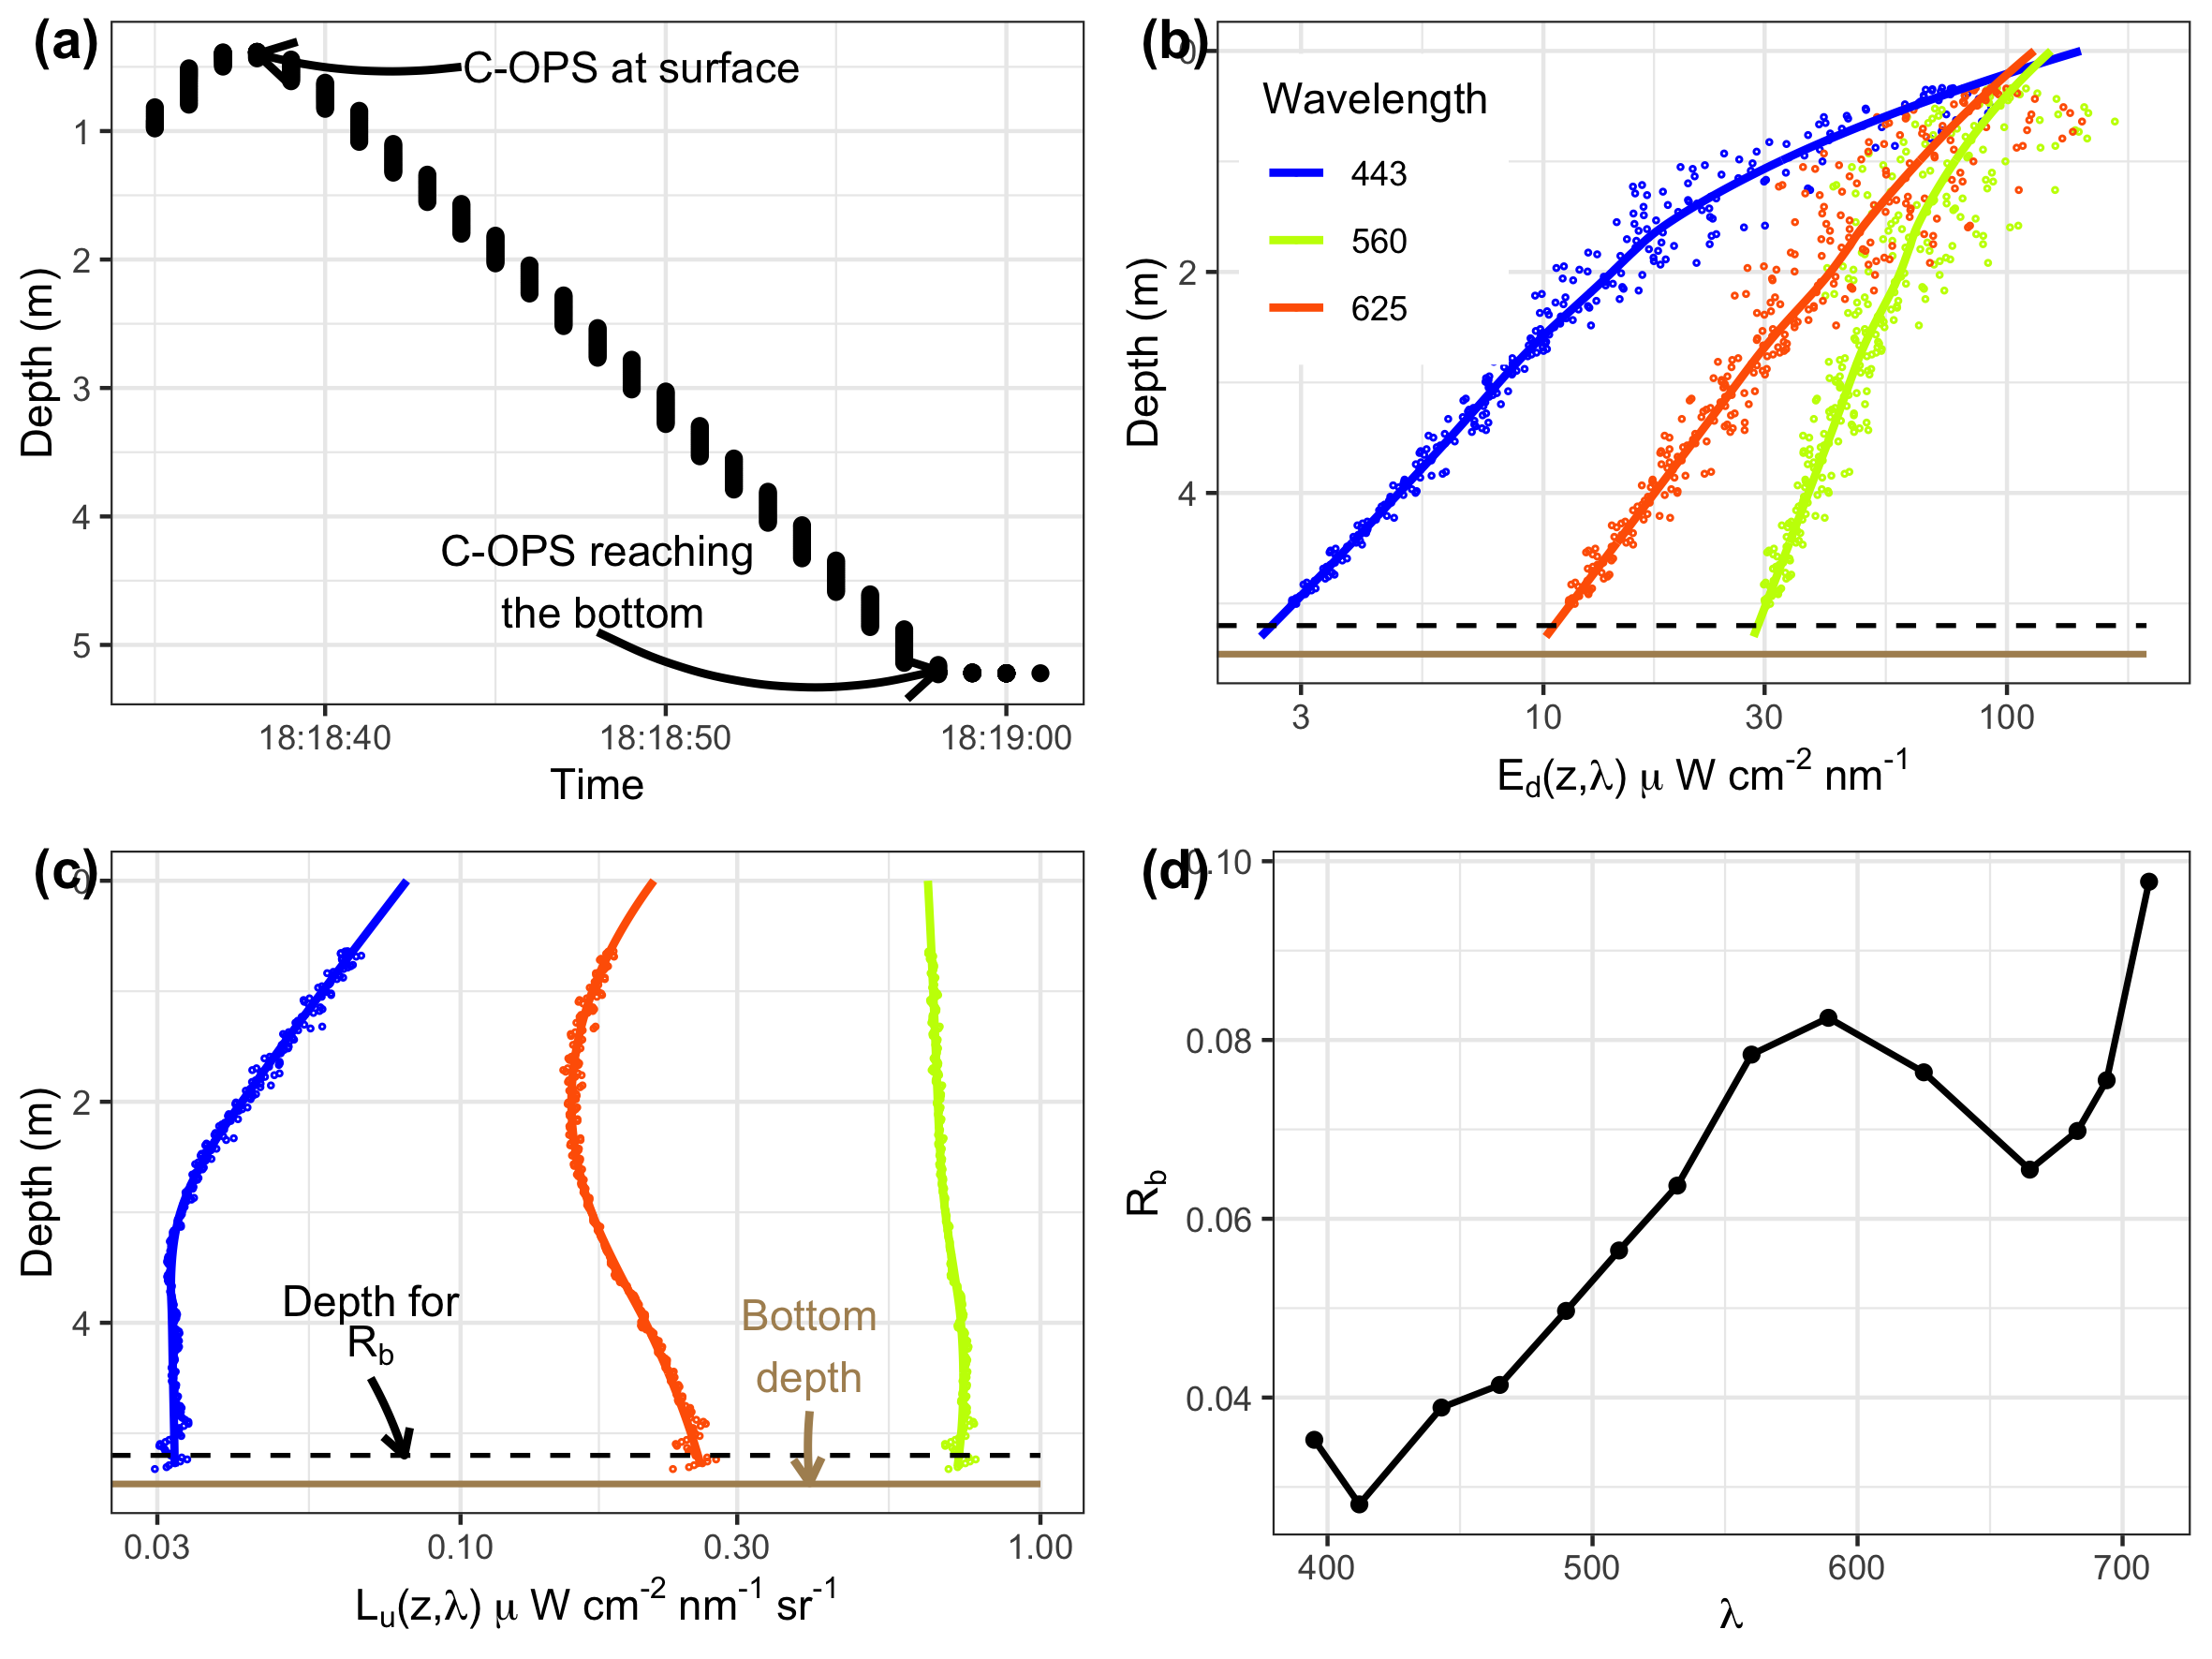
\includegraphics[width=18cm]{Figures/Fig_Rb.png}
    \caption{Example of an estimation of $R_b(\lambda)$  from C-OPS vertical profiles of $E_d(z,\lambda)$ and $L_u(z,\lambda)$, respectively.   }
    \label{fig:Rb}
\end{figure}
Figure~\ref{fig:Rb}d show $R_b(\lambda)$ of the MAN-F05 station as estimated using the average values derived from 3 C-OPS profiles. The spectral range $R_b(\lambda)$ in this example is restricted to 400 to 710 nm and determined by the detection limit of each individual C-OPS channel.\\       

\textbf{HyperOCR}\\

\subsubsection{Above-water radiometry}

\textbf{ASD}\\

\textbf{PSR-1100}\\

\subsubsection{Multiparametric and Inherent Optical Properties (IOPs)}
CTD, a-sphere, hydroscat, etc

\subsubsection{Sun photometry}
Sun photometry was determined for WISE-Man project only. Because the objective of WISE-Man was to determine the potential of hyperspectral imagery, the aerosol optical depth (AOD, dimensionless, spectral), Armstrong coefficient (dimensionless, indicating the spectral dependance of AODs) and precipitable water vapor (cm, measured from the 870 nm channel) were derived from measurements made with two handheld Microtops II (Solar Light Company) sun photometers during the project. Both instruments were calibrated by NASA prior to their deployment on separate vessels. These atmospheric parameters are useful for atmospheric radiative transfer applications (eg. climate studies), but in the context of ocean color radiometry, they are used to assess the contribution of the atmosphere to the reflected signal. For example, in NASA’s operational atmospheric correction processes, near infrared wavebands are used to assess the AOD of a scene (Bailey et al., 2010, OE, Gordon and Wang, 1994a, AO). This can lead to large uncertainties in glint correction, geophysical variable inversion over turbid waters, etc. (Werdell et al. 2018, PiO). To avoid this potentially important (and a priori unknown) error source in either space-borne or airborne high spatial resolution imagery recorded around the Manicouagan peninsula, these variables were derived from in situ measurements, allowing the atmospheric contribution to the surface reflectance to be properly characterized independently from the remote sensing imagery itself (Harmel et al. 2018, RSE).
 
During this field campaign, the atmospheric parameters were measured at 49 different instances, generally corresponding to different stations, with the exception of the Wise-Experiment for which six measurements were made at the same place but at different times. Here, one measurement refers to a series of scan replicates, five on average, to lower the uncertainties associated with operating the instrument from small vessels. The inversion of the signal was performed by AERONET using their Version 2 algorithm, with AOD uncertainties evaluated to be smaller than 0.02 at all wavelengths (Smirnov et al. 2009 JGR). Visual inspection of the AOD distributions per wavelength as well as spectral shape led to the removal of five suspect sequences for which only two or less scans were recorded and led to questionable values. 

\begin{figure}[t]
    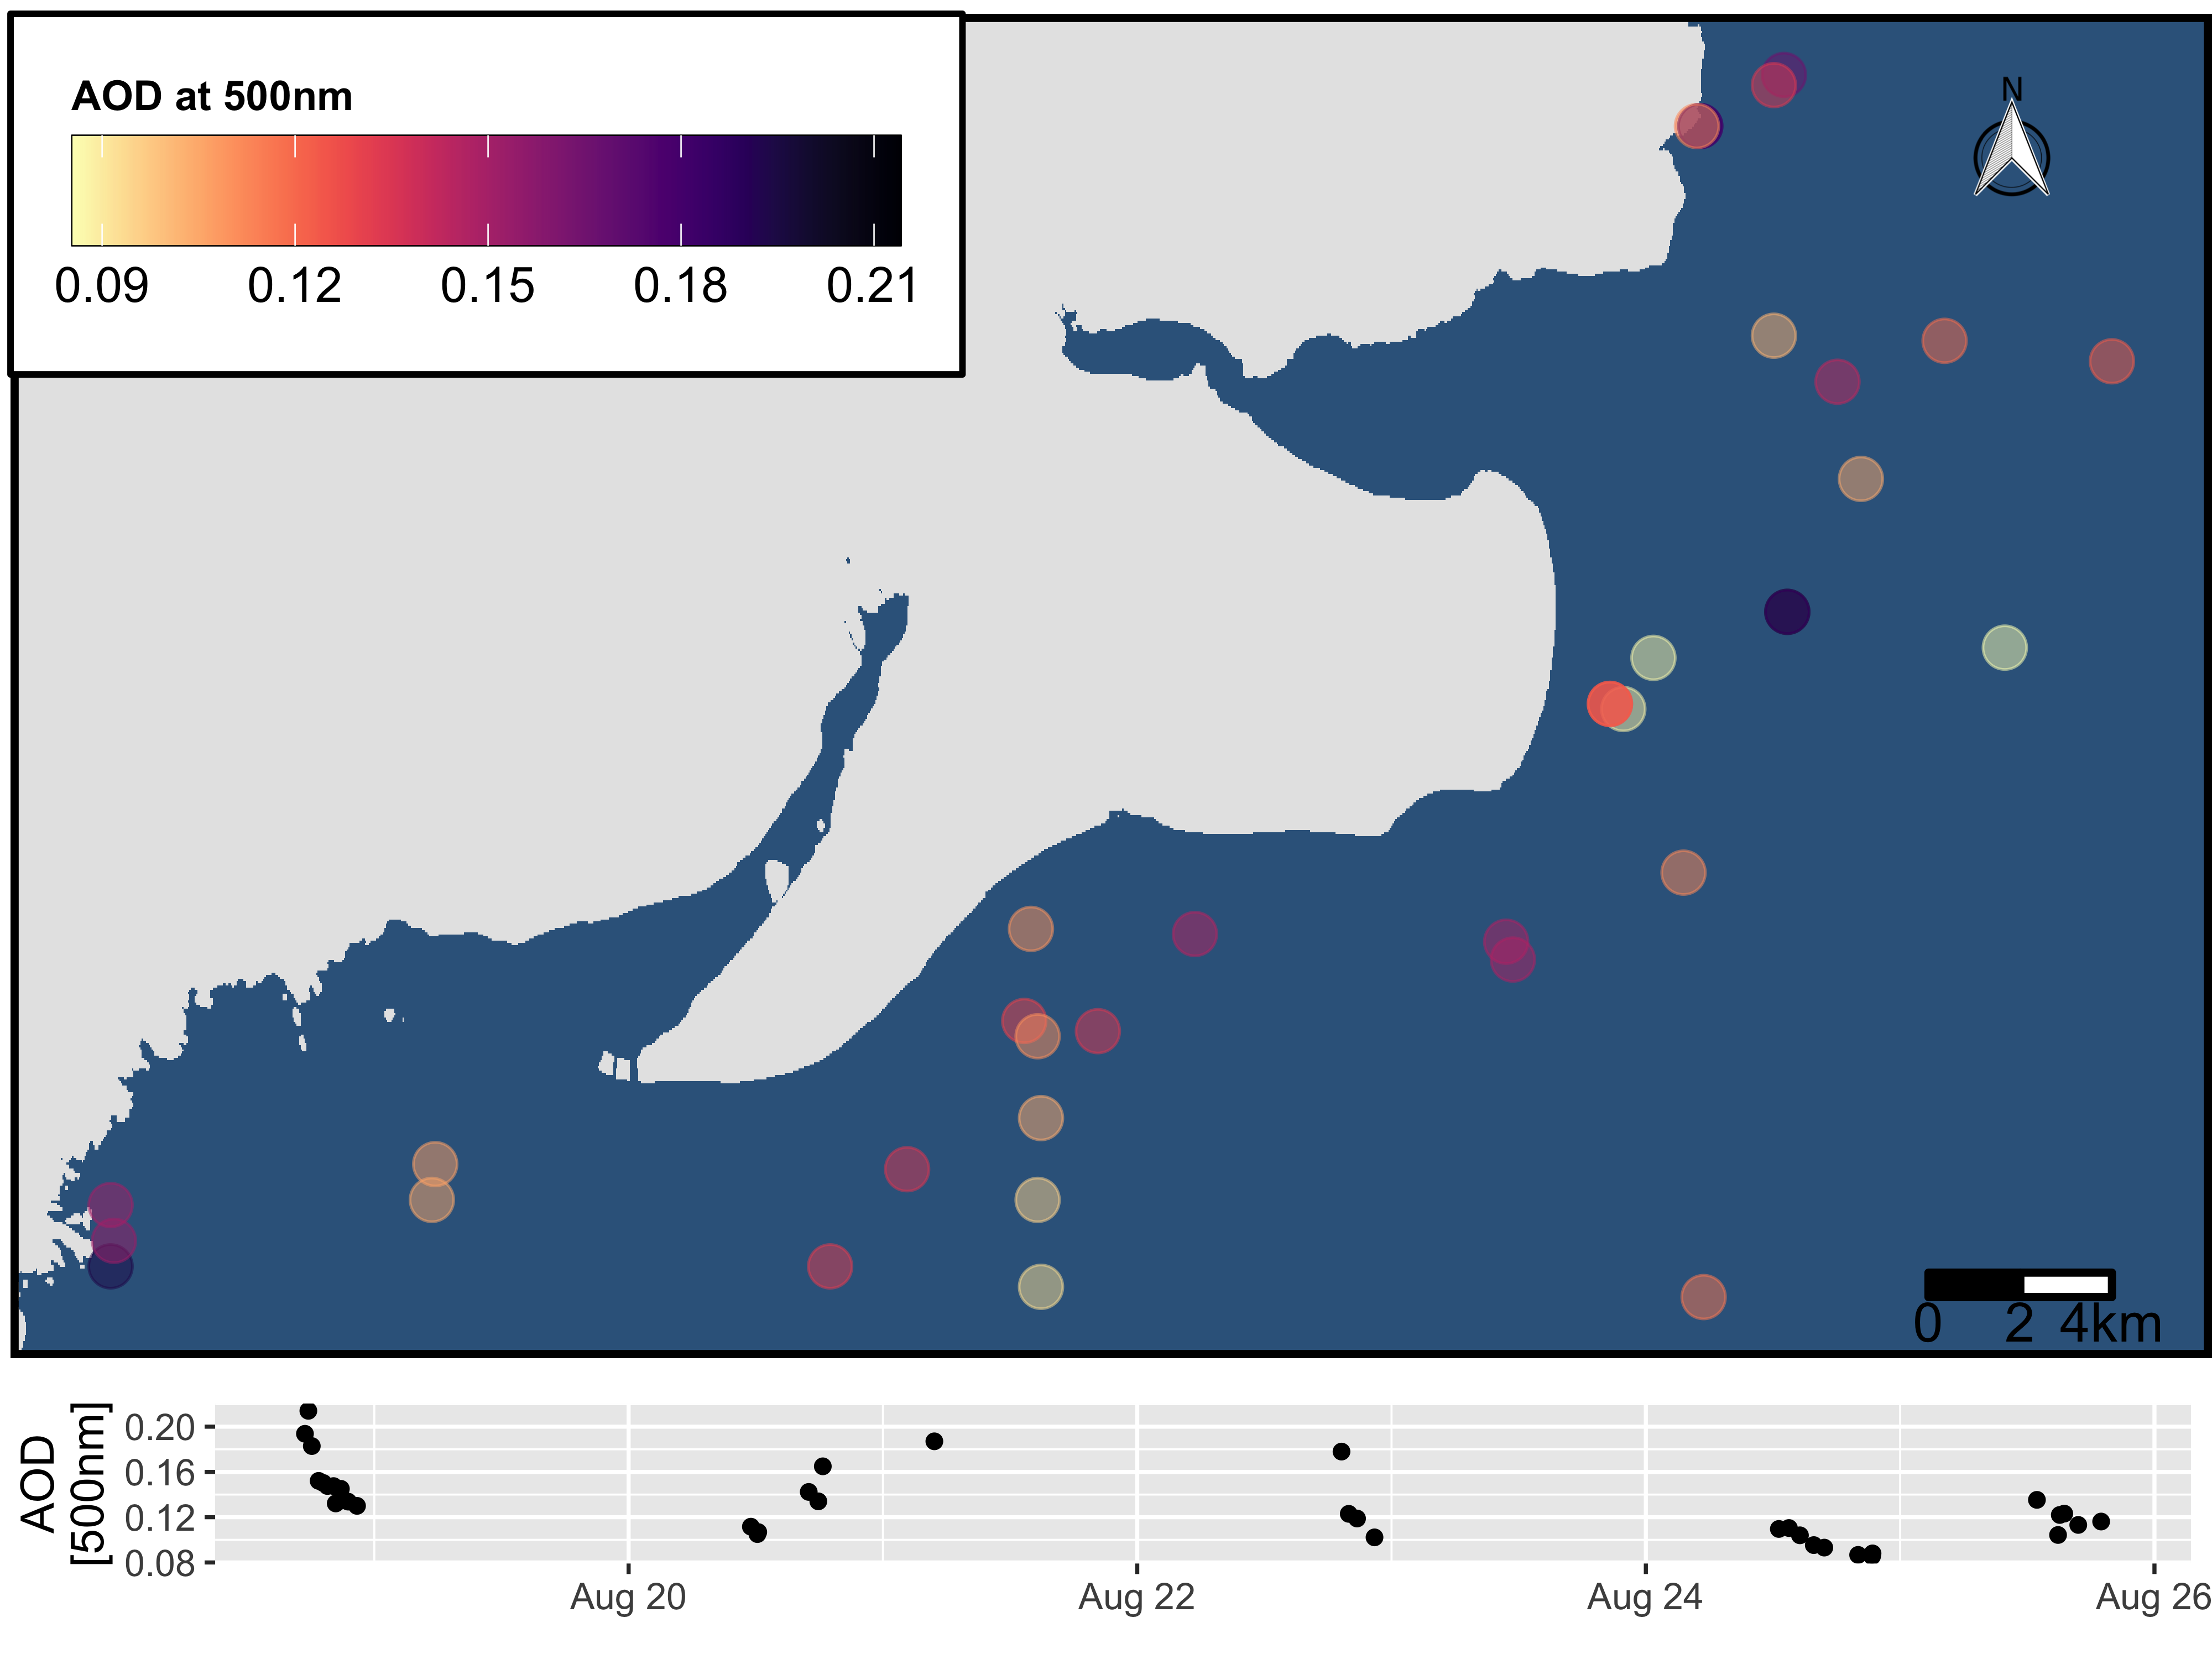
\includegraphics[width=8.3cm]{Figures/fig_AOD.png}
    \caption{Aerosol optical thickness at 500 nm between 17 and 25 August 2020 obtained from Microtops measurements made on two small vessels }
    \label{fig:AOD}
\end{figure}

 
Figure~\ref{fig:AOD} shows no discernible spatial pattern, but a decrease in AOD [500 nm] with time (WHY ? DO WE HAVE THE WIND DIRECTION ?). The median was computed for all the remaining sequences. A summary of these values is presented in Table \ref{table:AOT}. 
 

\begin{table}[t]
\caption{Summary of the atmospheric parameters derived from the two sun photometers.}
\centering
\begin{tabular}{ cccccc  }
\tophline
 & AOD [500nm] & AOD [870nm] & Angstrom exponent [440-870nm] & Water vapor (cm) & n\\
\middlehline
mean & 0.130 & 0.060 & 1.40 & 2.20 & 5.4 \\
std & 0.032 & 0.014 & 0.21 & 0.75 & 1.4 \\
min & 0.087 & 0.042 & 1.00 & 1.10 & 3.0 \\
max & 0.210 & 0.120 & 1.80 & 3.40 & 8.0 \\
\bottomhline
 \end{tabular}
 \label{table:AOT}
\end{table}

 
For perspective, over the deep ocean, Ahmad et al. (2010) mentioned typical AOD values at 870nm to around 0.086. Smirnov et al. (2009) found globally averaged oceanic AOD values of 0.108 at 500nm and 0.597 for the Angstrom exponent. Using all Maritime Aerosol Network data available in 2020 (https://aeronet.gsfc.nasa.gov/new\_web/maritime\_aerosol\_network.html), we split the dataset in coastal and oceanic data using a threshold of 100km from the nearest shore. For the coastal (oceanic) data, we found a mean AOD [500nm] of 0.151 (0.173), a mean AOD [870nm] of 0.090 (0.136) and a mean Angstrom exponent of 1.161 (0.609). In our case, all angstrom exponents were above one, representing a strong dominance of fine aerosols, continental in nature. Spectral shapes were monotonically decreasing towards longer wavelengths with an absence of blue-absorbing aerosols (Mobley et al. 2016).

\subsection{Laboratory analysis of discrete water samples} \label{labo}
Add details about how water was sampled/stored etc?
All together, the dataset contains xx water samples. Depending on the project and year of sampling, all or a subset of the following parameters were measured in the laboratory:

\subsubsection{Salinity}
Salinity (in PSU) was measured using a Guildline Portasal model 8410A salinometer. The average of three readings was taken as the final value.

\subsubsection{Nutrients}
Nutrients were made in ISMER for IML4 and by JET’s team (u.Laval) for CHONe and Wise.

\subsubsection{Spectrophotometric measurements}
CDOM absorption
CDOM absorbance OD(λ) was measured using the same method as described in Belanger et al. (2017). Seawater was filtered under low vacuum on 47 mm glass fiber filter (Whatman, GF/F 0.7 mm nominal pore size), which was pre-ashed for 2 h at 450℃ and pre-rinsed with 50 mL of MilliQ water. CDOM absorbance was measured with a Perkin Elmer double-beam Lambda-850 spectrophotometer using a 10 cm quartz cell between 220 and 800 nm against nano pure water. Absorption coefficients were then calculated according to:
\begin{equation}
%     aℊ(λ) = 2.303 OD(λ)/ι
a_g(\lambda) = \frac{2.303 OD(\lambda)}{L}
\label{eq:ag}
\end{equation}
where $a_g(\lambda)$ is the absorption coefficient of CDOM (m$^{-1}$) at wavelength $\lambda$, $OD$ is the absorbance measured at $\lambda$, and $L$ is the pathlength of the optical cell (0.1~m).

Particulate absorption
Measurements of particulate absorption were performed using the filter-pad technique, as described in Bélanger et al. (2017). A known volume of the water sample (in two to five replicates) was filtered through Whatman GF/F glass fiber filters shortly after sampling (< 3h). Each filter was then placed in the center of a 150 mm integrating sphere equipped with a spectralon filter holder (see Röttgers and Gehnke 2012 for technical details). The optical depth OD(λ) of the particles retained on the filter was then measured using a Perkin Elmer Lambda-850 spectrophotometer, from 300 to 800 nm at 1 nm resolution. Optical depth was converted to the spectral particulate absorption coefficient, ap(l)(m21), using

ap(λ) = 2.303 OD(λ) A/V OD(λ)-ODblank(λ)/β

where ODblank is the optical density of a blank filter, A is the clearance area of the particles on the filter (m2), V is the volume of sample water filtered (m3), and β is the pathlength amplification factor. The relationship between β and OD derived experimentally by Stramski et al. (2015) was used. After the OD scanning, phytoplankton pigments were extracted for 18–24h using methanol (Kishino et al. 1985), which removed nearly all pigments (95\% of sample). The filter was then placed again in the integrating sphere to measure the absorption coefficient of nonalgal particles, aNAP. The absorption coefficient of phytoplankton aø was obtained by subtracting aNAP from the total particulate absorption coefficient.

\subsubsection{ Chlorophyll-a and phaeo pigments: in vitro fluorometric determination}
Triplicate subsamples for Chl-a and phaeopigments concentration determination were filtered (varied volume) onto Whatman GF/F. Chl-a concentrations were measured using a Turner Designs 10-AU fluorometer, following a 24-h extraction in 90\% acetone at 4ºC in the dark without grinding (acidification method: Parsons et al. 1984). The final value from triplicates was determined considering their average, within a confidence interval of 95\%.

\subsubsection{Pigments: High Performance Liquid Chromatography (HPLC)}
Measurements of pigments were performed using High Performance Liquid Chromatography (HPLC) at ISMER, according to Zapata et al (2000). Water samples were filtered through 25 mm Whatman GF/F glass fiber filters (0.7 mm nominal pore size) and stored in cryogenic vials at -80℃. The internal standards (IS) of apo-caroten were stored at -20℃. The whole extraction procedure was conducted in the dark under a green light to avoid the degradation of the photosynthetic pigments. Samples were kept cool during the whole extraction procedure in an ice-filed container. Filters were placed in 15 ml tubes containing 3 ml of 95\% methanol. After letting the SI at room temperature for 5 minutes, a 50 µL volume was injected in the 15 ml tube containing the sample as well as in the blank sample. The samples were then crushed using a sonicator QSonica Q125 3 to 4 times at 5 seconds.  Once sonicated, the samples were centrifuged in a Eppendorf cooling centrifuge 5430R at 6500 RPM for 5 minutes at 4℃. Samples were filtered through a PTFE 0.2 mm encapsulated filter. The 13 mm capsule was screwed on a glass syringe and washed with acetone and methanol between each sample. The filtering step ensured to eliminate any impurities and kept only the relevant pigments to be analysed with HPLC. Finally, a small amount of argon was added to the vials in order to limit pigment oxidation caused by oxygen in the air.
 
Samples were placed in the HPLC analyser (Agilent Technologies 1 200 series) according to the method in Galindo et al. (2017) and the results were read with EzChrome Elite Software. A chromatogram representing the absorption peak of pigments in absorbance units (mAU) in relation to retention time (minutes) was generated for each sample. Detection and quantification limits were estimated as described in Bidigare et al. (2011). Peaks having an area under 2000 mAU were eliminated because of identification difficulties. Some pigments where standards were absent from our database were considered as “unknown” and discarded from future analyses. Those “unknows” were too scarce among the samples to allow proper identification. Reading of all pigments was done at 450 nm, except for phaeopigments, which were read at 412 nm because they are undetectable at 450 nm. A small variability was observed in retention time among the samples depending on the vial analyzed.
 
Pigment concentrations were calculated as follow:


CPig = (APig*Vex*Aapo\_blanc) / (C*Vinj*Vfil*Aapo\_ech)
 
where CPig is the individual pigment concentration (µg L–1), APig is the individual pigment peak area, Vex is the extraction total volume (mL), Aapo\_blanc is the apo-caroten peak area in the blank sample, C is the calibration coefficient associated with the pigment (area.µg–1), Vinj is the injected volume (mL), Vfil is the filtered volume (mL) and Aapo\_ech is the apo-carotene peak area in the sample.


\subsubsection{Bacterial and phytoplankton cells count: flow cytometry analysis}
Heterotrophic prokaryotes (Archaea and Bacteria) and <20 µm autotrophs abundances were measured by flow cytometry. For each analysis, duplicate 4 mL subsamples were fixed with glutaraldehyde Grade I (Sigma; 0.1\% final concentration) in the dark at room temperature for 15 min, flash-frozen in liquid nitrogen and then stored at -80°C until analysis. 
 
Samples for heterotrophic prokaryotes enumeration were stained with SYBR Green I (Invitrogen) following Belzile et al. (2008). Bacteria (and Archaea) were counted with a CytoFLEX flow cytometer (Beckman Coulter) using the blue laser (488 nm). The green fluorescence of nucleic acid-bound SYBR Green I was measured at 525 nm (525/40 nm BP). The cytograms obtained were analyzed using CytExpert v2.3 software and the same regions of the side scatter vs. green fluorescence plots were ascribed to low nucleic acid (LNA) and high nucleic acid (HNA) bacteria for the whole dataset.
 
Samples for <20 µm autotroph abundances (i.e. phycoerythrin-containing cyanobacteria, phycocyanin-containing cyanobacteria and autotrophic eukaryotes) were analyzed using a CytoFLEX flow cytometer (Beckman Coulter) fitted with a blue (488 nm) and a red laser (638 nm). Using the blue laser, forward scatter, side scatter, orange fluorescence from phycoerythrin (582/42 nm BP) and red fluorescence from chlorophyll (690/50 nm BP) were measured. The red laser was used to excite the red fluorescence of phycocyanin (660/20 nm BP). Polystyrene microspheres of 2 µm diameter (Fluoresbrite YG, Polysciences) were added to each sample as an internal standard. Pico- (<2 µm) and nano-autotrophs (2-20 µm) were discriminated based on a forward scatter calibration using algal cultures. Nano-sized autotrophs containing phycoerythrin or phycocyanin were ascribed to nanocyanobacteria but could have also been cryptophytes or rhodophytes (Kirk 1994).

\subsubsection{Suspended Particulate Matter (SPM)}
SPM were measured according to Bélanger et al. (2017). Known volumes (V) in liters of seawater (1 L, depending on turbidity) were filtered in triplicate through pre-ashed (1h at 450℃) and pre-weighed (mass M0,mg) 25 mm glass fiber filters (Whatman, GF/F 0.7 mm nominal pore size) at low vacuum (VanDer Linde 1998). Each filter was then rinsed with Milli-Qwater, dried for 24h at 60℃ prior to weighing under a dry atmosphere (mass M1, mg) to obtain the SPM concentration (mgL-1) as:

SPM =(M1 - M0) / V

Organic matter lost on ignition (LOI) was determined after baking the filters for 3h at 500℃, weighing again, giving the concentration of particulate inorganic matter (PIM).
The average coefficient of variation (CV) for triplicates considering the entire dataset is 17.95\% and 22.45\% respectively for SPM and PIM. CV for individual project are presented in Table (under).

\begin{table}[t]
\caption{Coefficient of variation for SPM and PIM.}
\centering
\begin{tabular}{ c|cc  }
\tophline
 & SPM & PIM\\
\middlehline
PMZA-RIKI & 20.21 & 23.71 \\
BSI & 15.70 & 18.79 \\
WISE-Man & 21.87 & 28.48 \\
\bottomhline
 \end{tabular}
 \label{table:SPMCV}
\end{table}

\subsubsection{Total and Dissolved Organic Carbon (TOC, DOC) and Nitrogen (TDN)}
DOC concentration was measured using a Shimadzu TOC-Vcpn carbon analyzer equipped with a TNM-1 module (Total Nitrogen Measurement unit) simultaneously measuring the dissolved nitrogen concentration (DN, inorganic plus organic). Potassium hydrogen phthalate and potassium nitrate were used to standardize DOC and DN measurements, respectively. In addition, samples were systematically checked every seventh sample analysis against Nanopure water (Barnstead Nanopure Infinity) and deep seawater reference from Florida Strait (43-45 µmol C L-1 and 32-33 µmol N L-1) produced by the Hansell’s consensus reference materials (CRM) program. The coefficient of variation on three replicate injections was typically <2\% for DOC and <5\% for DN.

\subsubsection{Phytoplankton taxonomy}

\subsection{Benthic habitats} \label{benthos}
\subsubsection{Surface reflectance}
The spectra of 195 stations were measured ten times over the vegetation-growing season from the 28th of july to the 7th of august (Table X). Those stations cover the principal component (Seagrass (Zostera Marina), macroalgae, saltmarsh cordgrass (Spartina alterniflora) and Mediterranenea saltbush (Atriplex halimus)) of the Manicouagan Peninsula (Figure X). The plot area was defined to cover a homogeneous part of each vegetation community. A full species composition description, with their percentage cover estimates, was made for every plot. At least 10 to 15 field spectrometer measurements were taken at random over the vegetation type on each homogeneous plot. This ensured that the random spectral measurements on each plot covered the range of variance within the homogeneous vegetation plot.
Surface reflectance was measure with a VIS-NIR spectroradiometer from the Analytical Spectral Device Inc, commonly referred to as the ASD. It is a portable spectroradiometer that measures the energy return of the light coming from the surfaces, absolute or relative. The model used in manipulating this experiment is the Handheld2-pro model, which covers wavelengths from 325 to 1075 nm. The ASD collects five spectra and then averages. In addition, a replica of each site is made to ensure the accuracy of the data. The stations were visite at low tide so all the acquisition were made on emerged surface. For the acquisition of emerged surface reflectance, the instrument fitted to a 5-m optical fiber having a field-of-view (FOV) of 25°. The fiber was installed at the end of a rod fixed to a tripod pointing the surface at the nadir at the right height the cover a 0.25 m2 surface. Before each surface reflectance measurement, a calibrated reference (spectralon plate) with known reflectance value was measured.

\subsubsection{Surface sediments}

\subsubsection{Vegetation characterization}

\section{Results}
Examples of plots to show the results. Note that there seem to have outliers here and there...

\begin{figure}[t]
    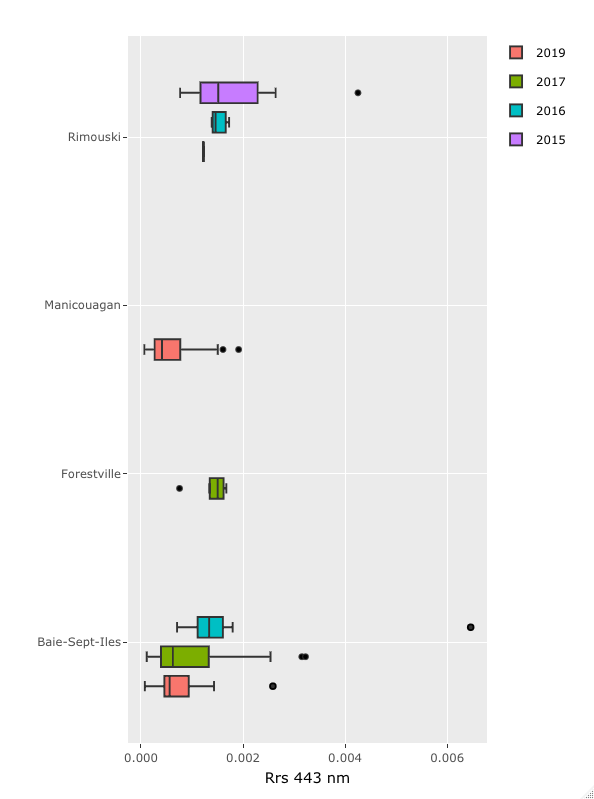
\includegraphics[width=8.3cm]{Figures/fig_RRs443_boxplot.png}
    \caption{The distribution of Rrs at 443 nm }
    \label{fig:Rrs443}
\end{figure}

\begin{figure}[t]
    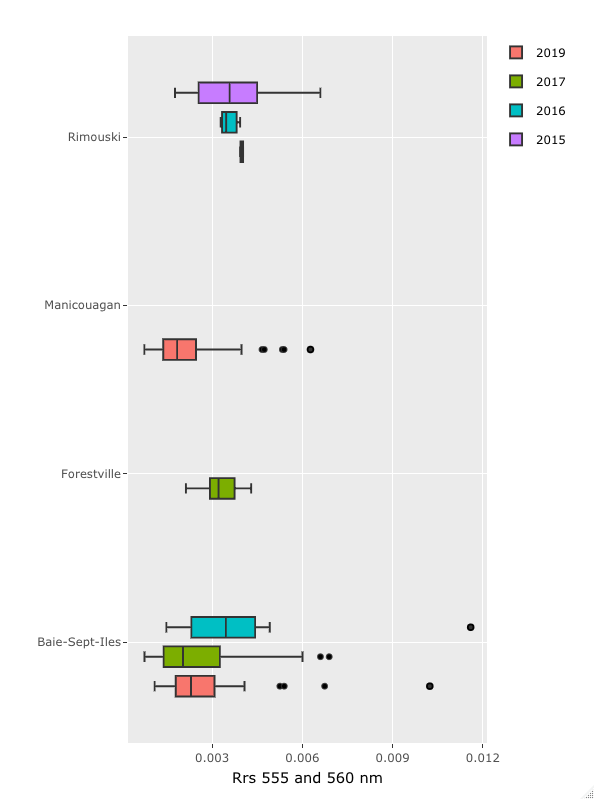
\includegraphics[width=8.3cm]{Figures/fig_Rrs555_boxplot.png}
    \caption{The distribution of Rrs at 555 and 560 nm }
    \label{fig:Rrs555}
\end{figure}

\begin{figure}[t]
    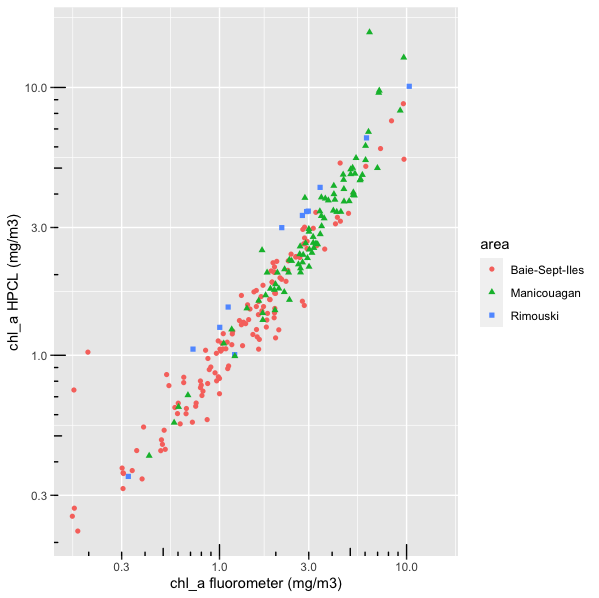
\includegraphics[width=8.3cm]{Figures/fig_regression_chla.png}
    \caption{Relationship between chlorophyll a concentration derived with different methods (HPLC and fluorometer), log-transformed to account for their log-normal distribution. }
    \label{fig:chlareg}
\end{figure}
\conclusions  %% \conclusions[modified heading if necessary]
TEXT

%% The following commands are for the statements about the availability of data sets and/or software code corresponding to the manuscript.
%% It is strongly recommended to make use of these sections in case data sets and/or software code have been part of your research the article is based on.

\codeavailability{TEXT} %% use this section when having only software code available


\dataavailability{TEXT} %% use this section when having only data sets available


\codedataavailability{TEXT} %% use this section when having data sets and software code available


\sampleavailability{TEXT} %% use this section when having geoscientific samples available


\videosupplement{TEXT} %% use this section when having video supplements available


\appendix
\section{Notation}    %% Appendix A
See Table in GDive and insert here once finished
https://docs.google.com/spreadsheets/d/1CQfSQyPWn0mrdXx9MKMdQom\_vfKphfoMwtqzOkksKIc/edit?usp=sharing

%% \subsection{}     %% Appendix A1, A2, etc.


\section{Additional Figures}\label{appendixfig}  
\begin{figure}
    \centering
    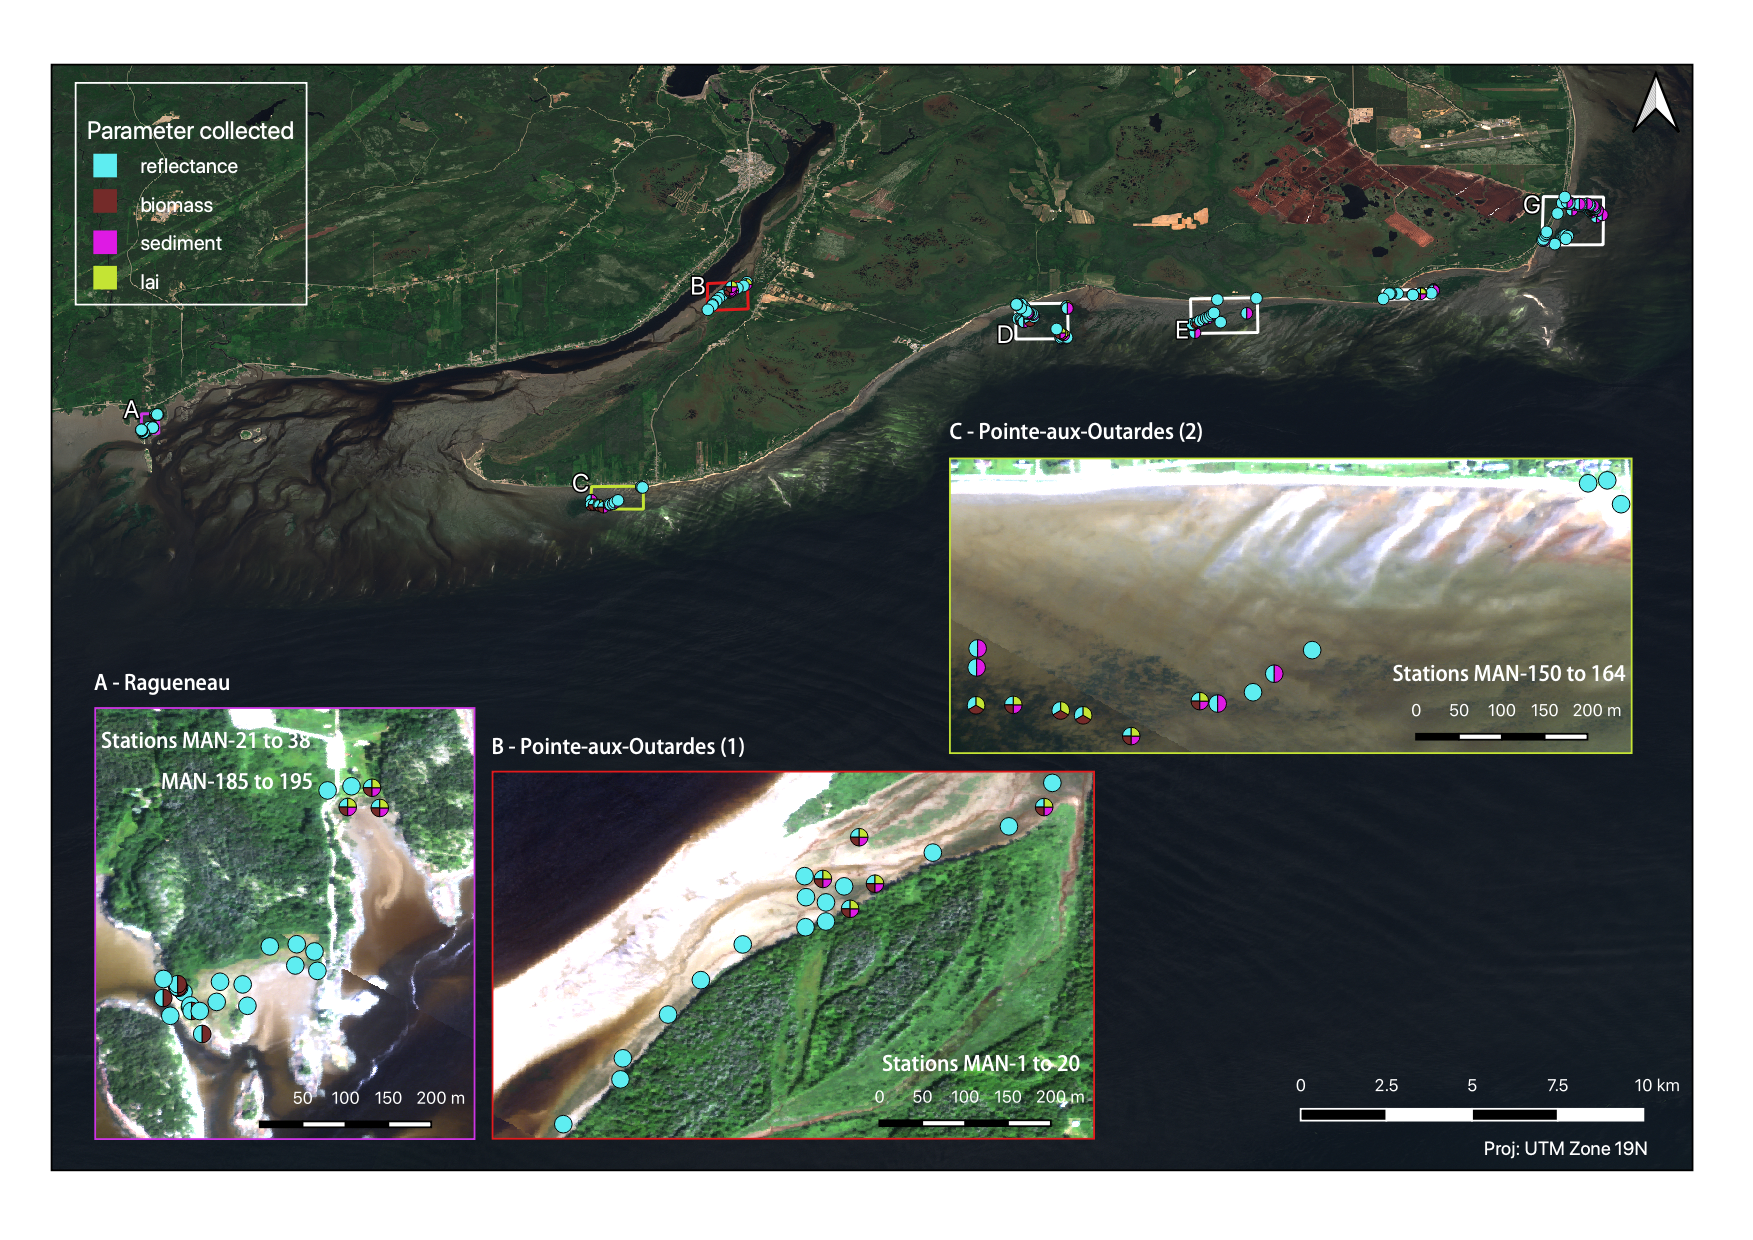
\includegraphics[width=18cm]{Figures/Fig2a_annexe_intertidal__A_B_C_v2.png}
    \caption{Map of stations in the inter-tidal zone visited at low tide between July 27 and August 8, 2019 in the Manicouagan peninsula, showing the different parameters sampled. Insets are zoomed in for three sectors (A, B and C) out of seven. }
    \label{fig:intertidal1_annexe}
    
\end{figure}

\begin{figure}
    \centering
    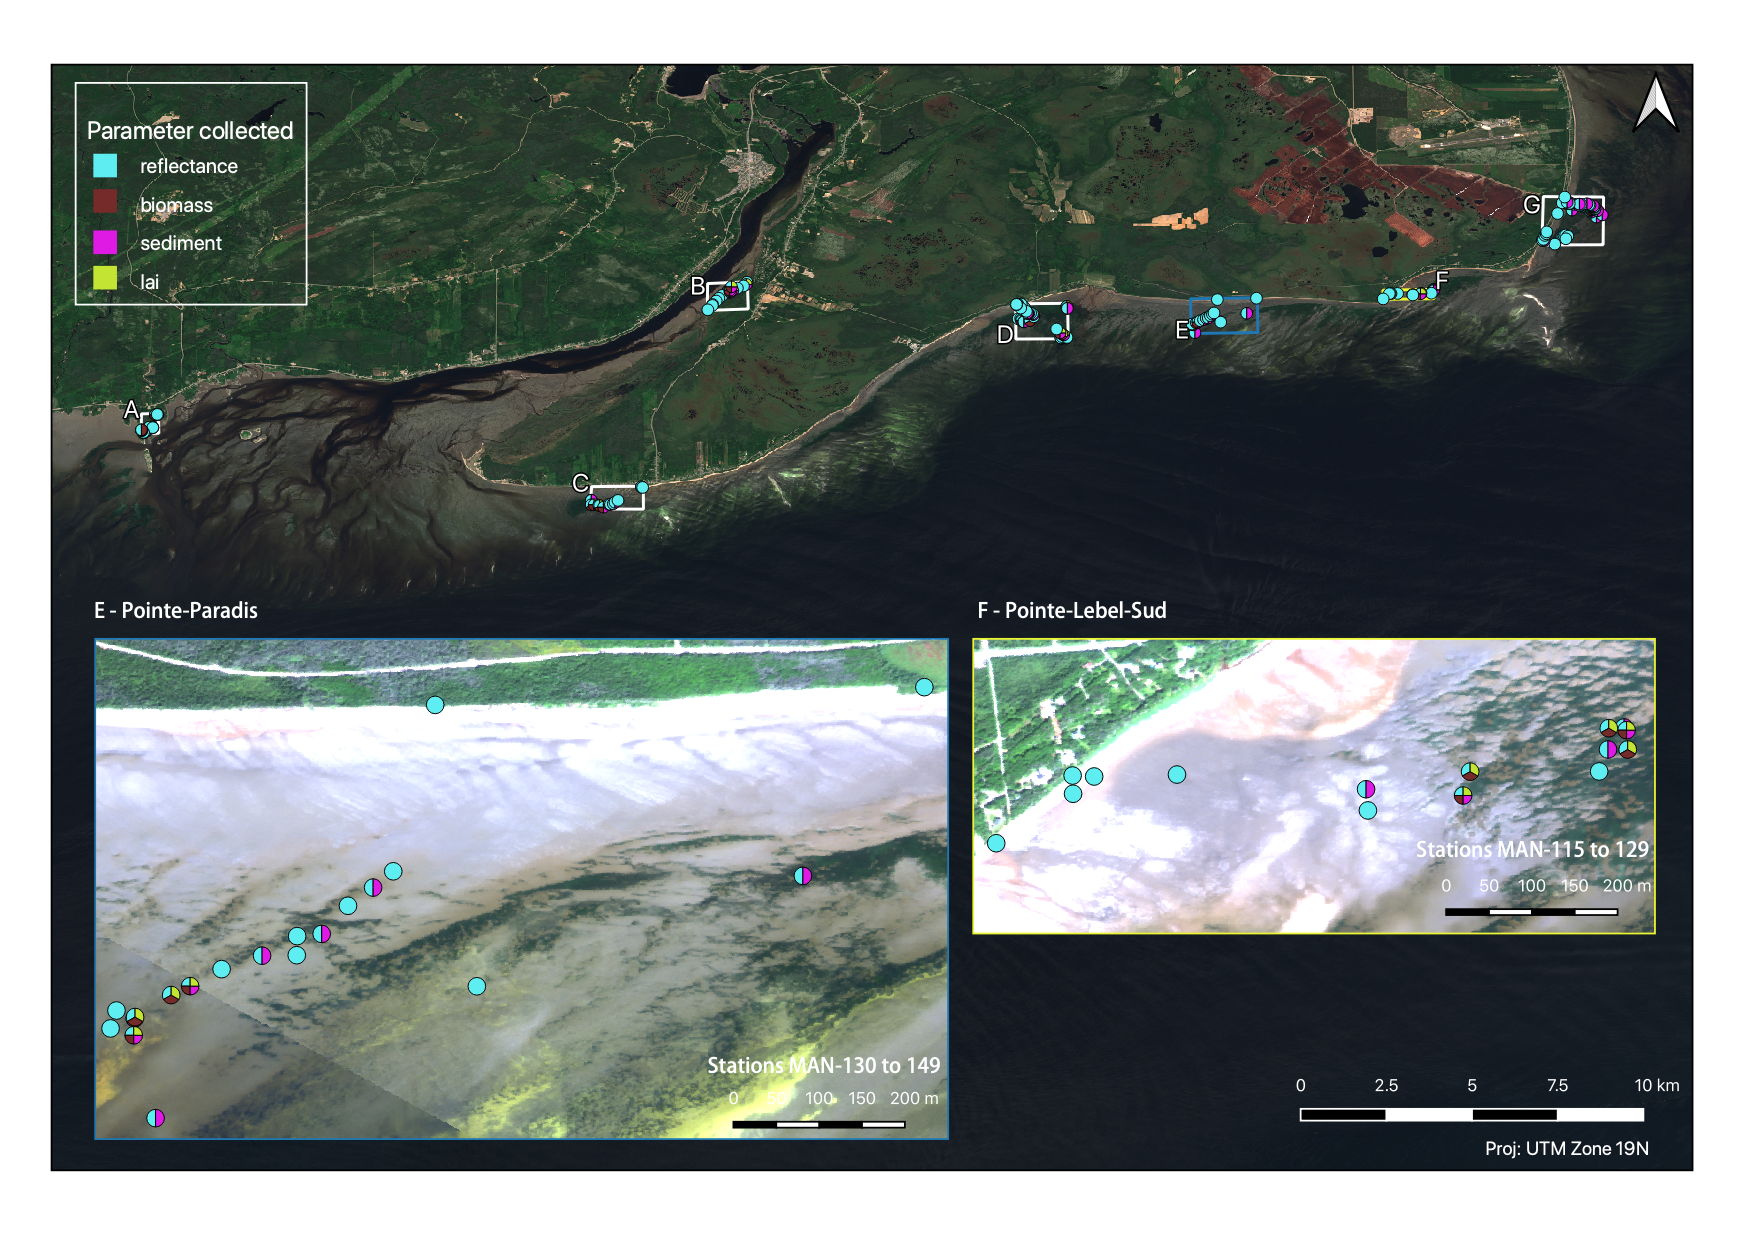
\includegraphics[width=18cm]{Figures/Fig2b_annexe_intertidal_E_F_v2.png}
    \caption{Map of stations in the inter-tidal zone visited at low tide between July 27 and August 8, 2019 in the Manicouagan peninsula, showing the different parameters sampled. Insets are zoomed in for two sectors (E and C) out of seven. }
    \label{fig:intertidal2_annexe}
\end{figure}

%% \subsection{}     %% Appendix A1, A2, etc.


\noappendix       %% use this to mark the end of the appendix section. Otherwise the figures might be numbered incorrectly (e.g. 10 instead of 1).

%% Regarding figures and tables in appendices, the following two options are possible depending on your general handling of figures and tables in the manuscript environment:

%% Option 1: If you sorted all figures and tables into the sections of the text, please also sort the appendix figures and appendix tables into the respective appendix sections.
%% They will be correctly named automatically.

%% Option 2: If you put all figures after the reference list, please insert appendix tables and figures after the normal tables and figures.
%% To rename them correctly to A1, A2, etc., please add the following commands in front of them:

\appendixfigures  %% needs to be added in front of appendix figures

\appendixtables   %% needs to be added in front of appendix tables

%% Please add \clearpage between each table and/or figure. Further guidelines on figures and tables can be found below.



\authorcontribution{TEXT} %% this section is mandatory

\competinginterests{TEXT} %% this section is mandatory even if you declare that no competing interests are present

\disclaimer{TEXT} %% optional section

\begin{acknowledgements}
TEXT
\end{acknowledgements}




%% REFERENCES

%% Since the Copernicus LaTeX package includes the BibTeX style file copernicus.bst,
%% authors experienced with BibTeX only have to include the following two lines:
%%
\bibliographystyle{copernicus}
\bibliography{references.bib}
%%
%% URLs and DOIs can be entered in your BibTeX file as:
%%
%% URL = {http://www.xyz.org/~jones/idx_g.htm}
%% DOI = {10.5194/xyz}


%% LITERATURE CITATIONS
%%
%% command                        & example result
%% \citet{jones90}|               & Jones et al. (1990)
%% \citep{jones90}|               & (Jones et al., 1990)
%% \citep{jones90,jones93}|       & (Jones et al., 1990, 1993)
%% \citep[p.~32]{jones90}|        & (Jones et al., 1990, p.~32)
%% \citep[e.g.,][]{jones90}|      & (e.g., Jones et al., 1990)
%% \citep[e.g.,][p.~32]{jones90}| & (e.g., Jones et al., 1990, p.~32)
%% \citeauthor{jones90}|          & Jones et al.
%% \citeyear{jones90}|            & 1990



%% FIGURES

%% When figures and tables are placed at the end of the MS (article in one-column style), please add \clearpage
%% between bibliography and first table and/or figure as well as between each table and/or figure.

% The figure files should be labelled correctly with Arabic numerals (e.g. fig01.jpg, fig02.png).


%% ONE-COLUMN FIGURES

%%f
%\begin{figure}[t]
%\includegraphics[width=8.3cm]{FILE NAME}
%\caption{TEXT}
%\end{figure}
%
%%% TWO-COLUMN FIGURES
%
%%f
%\begin{figure*}[t]
%\includegraphics[width=12cm]{FILE NAME}
%\caption{TEXT}
%\end{figure*}
%
%
%%% TABLES
%%%
%%% The different columns must be seperated with a & command and should
%%% end with \\ to identify the column brake.
%
%%% ONE-COLUMN TABLE
%
%%t
%\begin{table}[t]
%\caption{TEXT}
%\begin{tabular}{column = lcr}
%\tophline
%
%\middlehline
%
%\bottomhline
%\end{tabular}
%\belowtable{} % Table Footnotes
%\end{table}
%
%%% TWO-COLUMN TABLE
%
%%t
%\begin{table*}[t]
%\caption{TEXT}
%\begin{tabular}{column = lcr}
%\tophline
%
%\middlehline
%
%\bottomhline
%\end{tabular}
%\belowtable{} % Table Footnotes
%\end{table*}
%
%%% LANDSCAPE TABLE
%
%%t
%\begin{sidewaystable*}[t]
%\caption{TEXT}
%\begin{tabular}{column = lcr}
%\tophline
%
%\middlehline
%
%\bottomhline
%\end{tabular}
%\belowtable{} % Table Footnotes
%\end{sidewaystable*}
%
%
%%% MATHEMATICAL EXPRESSIONS
%
%%% All papers typeset by Copernicus Publications follow the math typesetting regulations
%%% given by the IUPAC Green Book (IUPAC: Quantities, Units and Symbols in Physical Chemistry,
%%% 2nd Edn., Blackwell Science, available at: http://old.iupac.org/publications/books/gbook/green_book_2ed.pdf, 1993).
%%%
%%% Physical quantities/variables are typeset in italic font (t for time, T for Temperature)
%%% Indices which are not defined are typeset in italic font (x, y, z, a, b, c)
%%% Items/objects which are defined are typeset in roman font (Car A, Car B)
%%% Descriptions/specifications which are defined by itself are typeset in roman font (abs, rel, ref, tot, net, ice)
%%% Abbreviations from 2 letters are typeset in roman font (RH, LAI)
%%% Vectors are identified in bold italic font using \vec{x}
%%% Matrices are identified in bold roman font
%%% Multiplication signs are typeset using the LaTeX commands \times (for vector products, grids, and exponential notations) or \cdot
%%% The character * should not be applied as mutliplication sign
%
%
%%% EQUATIONS
%
%%% Single-row equation
%
%\begin{equation}
%
%\end{equation}
%
%%% Multiline equation
%
%\begin{align}
%& 3 + 5 = 8\\
%& 3 + 5 = 8\\
%& 3 + 5 = 8
%\end{align}
%
%
%%% MATRICES
%
%\begin{matrix}
%x & y & z\\
%x & y & z\\
%x & y & z\\
%\end{matrix}
%
%
%%% ALGORITHM
%
%\begin{algorithm}
%\caption{...}
%\label{a1}
%\begin{algorithmic}
%...
%\end{algorithmic}
%\end{algorithm}
%
%
%%% CHEMICAL FORMULAS AND REACTIONS
%
%%% For formulas embedded in the text, please use \chem{}
%
%%% The reaction environment creates labels including the letter R, i.e. (R1), (R2), etc.
%
%\begin{reaction}
%%% \rightarrow should be used for normal (one-way) chemical reactions
%%% \rightleftharpoons should be used for equilibria
%%% \leftrightarrow should be used for resonance structures
%\end{reaction}
%
%
%%% PHYSICAL UNITS
%%%
%%% Please use \unit{} and apply the exponential notation


\end{document}
